%! suppress = Makeatletter
%! suppress = Makeatletter
\documentclass[11pt]{report}

\usepackage[T1]{fontenc}
\usepackage[utf8]{inputenc}
\usepackage{graphicx}
\usepackage{amsmath,amssymb,amsfonts}
\usepackage{polski}
\usepackage[raggedright]{titlesec}
\usepackage{indentfirst}
\usepackage{listings}
\usepackage{hyperref}
\usepackage[backend=biber, bibencoding=utf8, style=ieee, dashed=false, isbn=false, doi=false, sorting=anyvt]{biblatex}
\usepackage{caption}
\captionsetup{%
justification=raggedright,
labelfont=bf,
singlelinecheck=off
}

\DeclareUnicodeCharacter{0327}{}
\DeclareUnicodeCharacter{25CC}{}

%\addbibresource{library.bib}
\addbibresource{NEW.bib}

\pagestyle{headings}

\renewcommand{\chaptername}{Rozdział}
\renewcommand{\contentsname}{Spis treści}
\renewcommand{\figurename}{Rys.}
\renewcommand{\tablename}{Tab.}
\renewcommand{\listfigurename}{Spis rysunków}
\renewcommand{\listtablename}{Spis tabel}
\renewcommand{\bibname}{Bibliografia}

\makeatletter
\renewcommand{\l@section}{\@dottedtocline{1}{1.5em}{2.6em}}
\renewcommand{\l@subsection}{\@dottedtocline{2}{4.0em}{3.6em}}
\renewcommand{\l@subsubsection}{\@dottedtocline{3}{7.4em}{4.5em}}
\makeatother

\begin{document}
    \begin{titlepage}
        \centering
        
\includegraphics[width=\linewidth]{fig/AGH.jpg}
        \center{\scshape WYDZIAŁ INFORMATYKI, ELEKTRONIKI\\ i~TELEKOMUNIKACJI}
        \vspace{0.03\textheight}
        \center{\textbf PRACA DYPLOMOWA MAGISTERSKA}
        \vspace{0.03\textheight}
        \center{\LARGE\bfseries Agentowe środowisko do sterowania procesem identyfikacji i analizy wzorców czasowych w~notkach o zdarzeniach politycznych}
        \center{Multi-agent environment for management of the process of identifying and~analyzing time patterns in news about political events}
        \vspace{0.12\textheight}
        \begin{tabbing}
            \hspace{0.3\textwidth}\=\\
            Autor: \>Michał Patyk\\
            Kierunek studiów:\> Informatyka\\
            Opiekun pracy:\> dr hab.
            inż.
            Jarosław Koźlak
        \end{tabbing}
        \vspace{0.04\textheight}
        \center{Kraków 2021}
%        TODO: remove next line
        \center{wersja 0.1.5}
    \end{titlepage}

    \tableofcontents


    \chapter{Wstęp}\label{ch:wstęp}


    \chapter{Przegląd dziedziny}\label{ch:przegląd-dziedziny}
    W tym rozdziale w części~\ref{subsec:gdelt} opisany został zbiór GDELT\@.


    \section{Wzorce}

    \subsection{Ogólne}

    \subsubsection{Wzorce w sieciach społecznościowych}
    W pracy~\cite{10.1093/jigpal/jzaa042} autorzy identyfikują i kategoryzują wzorce opisujące interakcje między użytkownikami w sieciach społecznościowych.
    Uwaga została skupiona na wzorcach w których występują częste interakcje dwóch lub więcej użytkowników oraz na pozycji społecznej tych użytkowników w sieci.
    Zbiór danych został podzielony na N okien czasowych.
    Lista postów była eksportowana dla każdego okna, a na jej podstawie tworzono słownik.
    Przy pomocy słownika analizowano relacje miedzy użytkownikami.

    W pracy Odkrywanie ukrytych informacji w mediach społecznościowych~\cite{Skwara2019} autor bada częste lub nietypowe wzorce zachowań użytkowników mediów społecznościowych.
    Wzorce: wierny komentator, cięty komentator, dwaj komentatorzy, dwóch na jednego, komentator dwóch autorów, czujny komentator, prawo przechodniości.

    \subsection{GDELT}\label{subsec:gdelt}
    Celem pracy~\cite{Jarosz2020} identyfikacja wzorców w GDELT oraz opracowanie i ewaluacja algorytmów oraz metod analizy wzorców z tego zbioru\@.
    Badane wzorce zostały podzielone na statyczne oraz dynamiczne.
    Głównymi wyszczególnionymi elementami relacji sa powtarzalność oraz intensywność.
    Wzorce statyczne: sojusznik, nieprzyjaciel, symetria, asymetria, istotność, mocarstwo-klient.
    Wzorce dynamiczne: stabilna relacja, jedyna zmiana, pojedyncze zaburzenie, oscylacja, wzajemność, podobny ciąg dopasowań, zależność w czasie.
    Dodatkowe wzorce dynamiczne COVID-19: spadek nastrojów, nowa normalność, gratulacje, skupienie na walce.


    \section{Zastosowania}
    W pracy~\cite{Yan2012} autorzy proponują framework oparty na ważności dla charakteryzowania i wyodrębniania zmieniających sie wzorców w sieciach przedstawiających notatki prasowe.
    Zdefiniowano dwa wskaźniki istotności, aby scharakteryzować ewolucję i odkryć zmiany topologii o doniosłym znaczeniu.
    Cały proces znajdowania zachowań dynamicznych jest kierowany przez punktację istotności.

    \subsection{inne}\label{subsec:inne}
    Do analizy~\cite{Buckingham2020,Levin2018,Yuan2017}.


    \section{Systemy Agentowe}
    Według definicji z książki Grharda Weissa Systemy Wieloagentowe~\cite{55066420130101} agent to system komputerowy który jest umieszczony w pewnym środowisku i jest zdolny do autonomicznych akcji w tym środowisku w celu osiągnięcia wyznaczonych mu celów.
    Rysunek~\ref{fig:agent} przedstawia agenta w jego środowisku.
    \begin{figure}[!htp]
        \centering
        \includegraphics[width=\linewidth]{fig/agent_środowisko_weiss.png}
        \caption{Agent w swoim środowisku. (źródło: Multiagent Systems~\cite{55066420130101})}
        \label{fig:agent}
    \end{figure}
    Główną różnicą między agentami i obiektami jest stopień autonomiczności.
    Agenci nie wykonują nawzajem swoich metod ale raczej żądają wykonania czynności.
    Są zdolni reagowania, proaktywności i zachowań społecznych.
    Agent na podstawie swoich przekonań podejmuje najlepsze według niego decyzje.

    \subsection{Zalety Systemu Wieloagentowego}
    Główną zaletą wykorzystania systemu agentowego według Gerharda Weissa~\cite{55066420130101} jest możliwość samodzielnego decydowania przez system o tym co powinien zrobić w celu osiągnięcia celów mu wyznaczonych.
    Agenci którzy mogą działać w zmieniającym się, nieprzewidywalnym środowisku gdzie wykonywane akcje mogą się nie powieść nazywani są agentami inteligentnymi.
    Kolejna zaletą SA jest utrzymywanie równowagi między skupieniem na celu i reagowaniem na bodźce.
    Możliwość negocjacji i kooperacji.

    Obiekt nie jest zdolny do proaktywnego zachowania i nie jest w stanie samodzielnie decydować, co zrobić w określonej sytuacji.
    Autonomiczne komponenty oddelegowane do własnej kontroli mogą zostać wzbogacone o wyrafinowane umiejętności społeczne, to znaczy zdolność do podejmowania decyzji o zakresie i naturze ich interakcji w czasie wykonywania oraz inicjowania interakcji w sposób elastyczny (np. poprzez wyszukiwanie i negocjowanie świadczenia usług oraz dostarczania danych).


    \section{Metodologie rozwoju Systemu Agentowego}
    Dziedzina inżynierii oprogramowania zorientowanej na agentów zajmuje się opracowywaniem systemów opartych na agentach oraz sposobami wspierania ich rozwoju.
    W szczególności ma na celu dostarczenie metodologii projektowania systemów agentowych oraz narzędzi pomocniczych.

    \subsection{RIO}
    W pracy~\cite{S095741740200070220020101} autorzy proponują metodologię RIO (Roles, Interactions and Organizations) jako właściwe podejście przy analizie i projektowaniu systemów wieloagentowych.
    \begin{figure}[!ht]
        \centering
        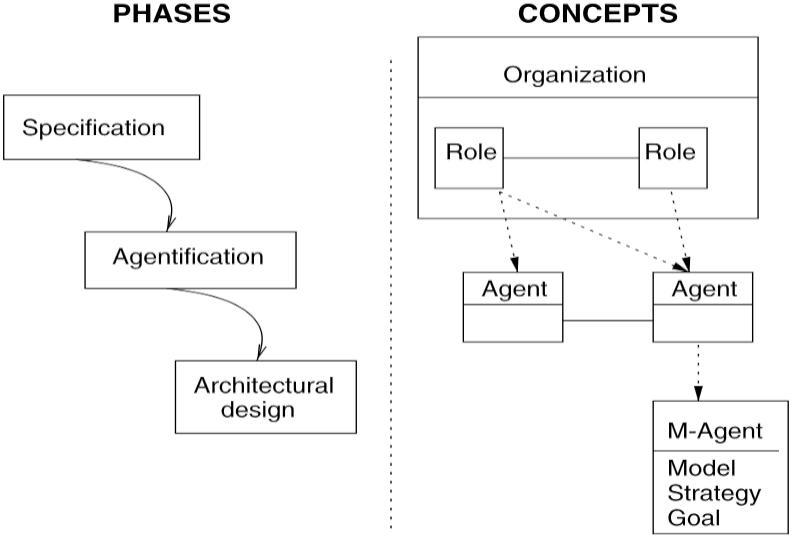
\includegraphics[width=\linewidth]{fig/RIO approach.png}
        \caption{Proces rozwoju w metodologii RIO. (źródło: A formal framework for multi-agent systems analysis and design \cite{S095741740200070220020101})}
        \label{fig:rio}
    \end{figure}
    System jest postrzegany jako organizacja która składa się ze zbioru wchodzących w interakcję ról.
    Role złożone powinny być dekomponowane na prostsze.
    Proces projektowania, przedstawiony na rysunku~\ref{fig:rio}, składa się z dwóch etapów: agentyfikacji i projektowania architektonicznego.
    Agentyfikacja to przypisanie roli do agentów.
    Na tym etapie nie robi się założeń co do architektury agentów.
    Dopiero etap projektowania architektonicznego kładzie naciska na wewnętrzną architekturę agenta.

    \subsection{GAIA}
    W pracy~\cite{Wooldridge2000a} autorzy opisują metodologię analizy i projektowania systemu agentowego Gaia
    Została ona założona na bazie widzenia systemu wieloagentowego jako organizacji obliczeniowej składającej się z wielu oddziałujących ze sobą ról.
    Proces analizy i projektowania, przedstawiony na rysunku~\ref{fig:gaia}, może być postrzegany jako przyrostowe budowanie coraz bardziej złożonych modeli systemu który ma być stworzony.
    \begin{figure}[!ht]
        \centering
        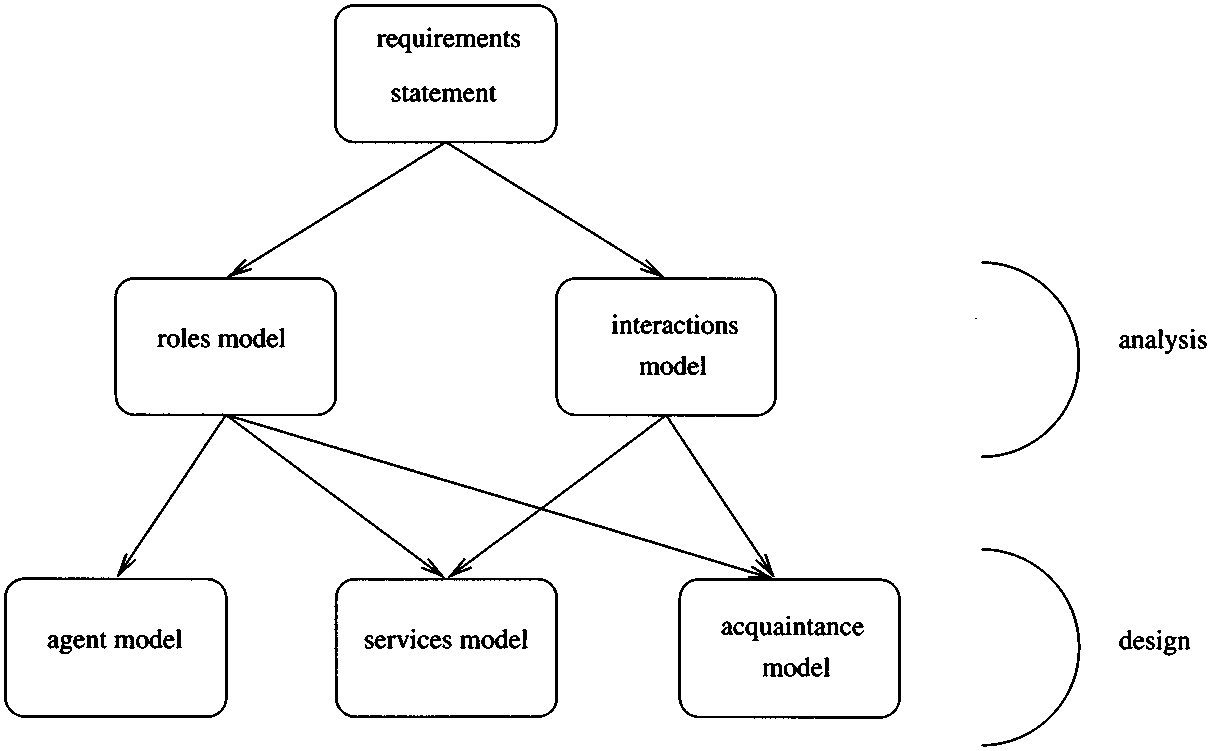
\includegraphics[width=\linewidth]{fig/gaia models.png}
        \caption{Zwiazek pomiędzy modelami Gaia. (źródło: The Gaia Methodology for Agent-Oriented Analysis and Design~\cite{Wooldridge2000a})}
        \label{fig:gaia}
    \end{figure}
    Celem etapu analizy jest rozwinięcie zrozumienia systemu i jego struktury.
    Podczas etapu projektowania Gaia skupia się na tym jak agenci mają kooperować aby zrealizować cele systemu oraz czego wymaga się od każdego agenta aby to osiągnąć.

    \subsection{GAIA v2}
    GAIA v2 jest oficjalnym rozszerzeniem metodologii.
    Role i protokoły są uzupełnione o środowisko, w którym działają agenci, specyfikujące jednostki i zasoby.
    Dodatkowe abstrakcje organizacyjne zostały przedstawione na rysunku~\ref{fig:gaia_v2}.
    \begin{figure}[!ht]
        \centering
        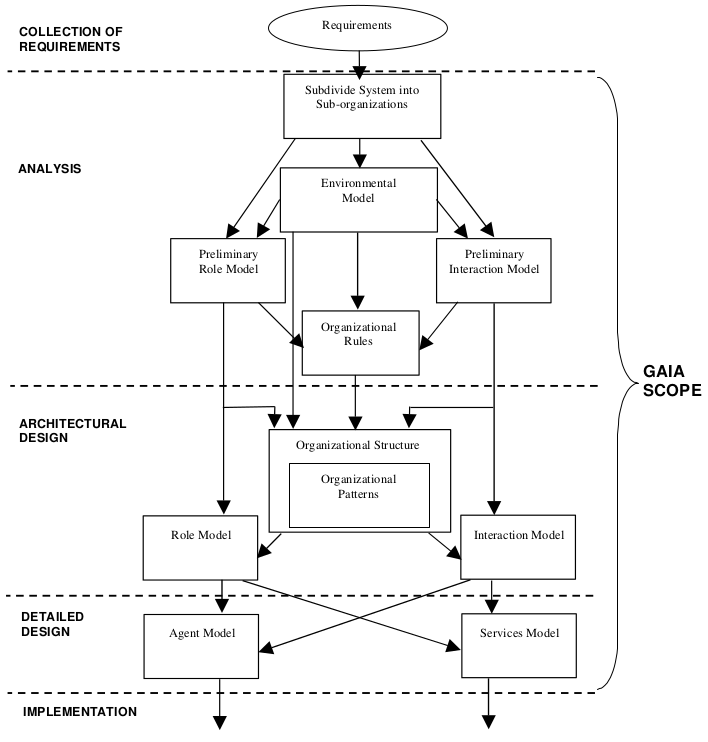
\includegraphics[width=\linewidth]{fig/gaia2 models.png}
        \caption{Modele i związki w GAIA v2. (źródło: Developing Multiagent Systems: The Gaia Methodology~\cite{Zambonelli2003})}
        \label{fig:gaia_v2}
    \end{figure}
    Reguły organizacyjne to ograniczenia które muszą być uwzględnione w globalnym zachowaniu organizacji.
    Struktura organizacyjna określa ogólną architekturę systemu.

    \subsection{ROADMAP}
    ROADMAP jest kolejnym rozszerzeniem metodologii GAIA.
    Faza analizy jest rozszerzona tak by pokryć również specyfikację.
    Wprowadzono dodatkowe modele opisujące środowisko oraz wiedze agentów.
    Rysunek~\ref{fig:roadmap} przedstawia strukturę modeli ROADMAP.
    \begin{figure}[!ht]
        \centering
        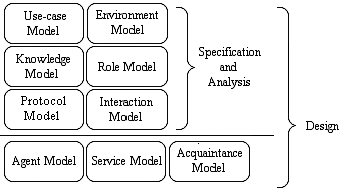
\includegraphics[width=\linewidth]{fig/roadmap models.png}
        \caption{Struktura modeli ROADMAP. (źródło: ROADMAP: Extending the Gaia methodology for complex open systems~\cite{Juan2002a})}
        \label{fig:roadmap}
    \end{figure}
    Hierarchia ról pełni podobną role do struktury i ról organizacyjnych w GAIA v2.
    Pozwala określić właściwe zachowanie agentów.

    \subsection{INGENIAS}
    W pracy~\cite{Pavon2003} autorzy przedstawiają metodologię rozwoju systemu wieloagentowego INGENIAS.
    Została ona zaprojektowana z myślą o budowie specyfikacji przyrostowo z zapewnieniem poprawności rozwoju.
    INGENIAS ulepsza oryginalne podejście z MESSAGE/UML poprzez dodanie nowego widoku oraz dostarczenie narzędzi do generowania kodu i dokumentacji systemu automatycznie ze specyfikacji.
    Generalnym podejściem INGENIAS do specyfikacji systemu wieloagentowego jest podział problemu na aspekty które tworzą różne widoki systemu.
    Każdy rodzaj widoku jest opisany z wykorzystaniem języka meta-modelującego.
    INGENIAS wyróżnia pięć metamodeli opisujących widoki, które muszą zostać wykorzystane przy opisie systemu:
    \begin{enumerate}
        \item Model agenta który opisuje pojedynczego agenta, jego zadania, cele, początkowy stan oraz role,
        \item Model interakcji który opisuje jakie interakcje mogą zajść między agentami,
        \item Model zadań i celów który opisuje relację między zadaniami i celami oraz ich strukturami,
        \item Model organizacji który opisuje jak komponenty systemu są ze sobą pogrupowane, jakie ograniczenia istnieją w interakcjach między agentami,
        \item Model środowiska który definiuje postrzeganie agentów jako elementów systemu oraz identyfikuje zasoby systemu.
    \end{enumerate}

    \subsection{Wnioski z przeglądu metodologii}
    \ldots


    W pracy z 2001 roku~\cite{Smirnov2002} autorzy przedstawiają technologię systemów wieloagentowych jako podstawę systemów Fuzji Wiedzy.
    Fuzje Wiedzy można zdefiniować jako integrację luźno powiązanych źródeł w połączone zasoby w celu uzupełnienia niedostatecznej wiedzy i uzyskania nowej.
    Korzystanie z inteligentnych agentów zwiększa wydajność i interoperacyjność systemu ponieważ agenci mogą działać w środowisku rozproszonym, niezależnie od użytkownika, i wykorzystywać
    ontologie do reprezentacji i wymiany wiedzy.


    \chapter{Koncepcja}\label{ch:koncepcja}
    Identyfikacja wzorców: opisujących państwa oraz relacje między państwami.
    Stworzenie reguł wspomagających odnajdywanie wzorców.

    Wejściem systemu jest zadanie konfiguracyjne.
    Zadanie konfiguracyjne uruchamia system który szuka wzorców.
    System zajmuje się:
    \begin{enumerate}
        \item rozdziałem zadań dla agentów,
        \item wyszukiwaniem wzorców,
        \item zbieraniem danych,
        \item analizą,
        \item generowaniem zestawień.
    \end{enumerate}

    Grupy agentów profilowane w celu automatycznego wyszukiwania wzorców czasowych.
    Zróżnicowanie agentów obejmuje:
    \begin{enumerate}
        \item progi,
        \item poziomy granulacji,
        \item wyszukiwanie korelacji,
        \item wyszukiwanie trendów,
        \item wykorzystanie dodatkowych źródeł informacji.
    \end{enumerate}

    Na wyjściu systemu otrzymujemy zagregowane dane.


    \section{Miary}\label{sec:miary}
    Miary jakie zostaną wykorzystane do poszukiwania wzorców:
    \begin{enumerate}
        \item[•] liczby zdarzeń w~analizowanym okresie, w~których dany kraj jest aktorem 1 (dalej oznaczone jako \textit{Events}),
        \item[•] sumy liczby wzmianek (całkowitej liczby wzmianek o~tym wydarzeniu, we wszystkich dokumentach źródłowych podczas 15-minutowej aktualizacji, w~której zostało po raz pierwszy zauważone) w~analizowanym okresie, dla wydarzeń w~których dany kraj jest aktorem 1 (dalej oznaczone jako \textit{numMentions}),
        \item[•] stosunku liczby zdarzeń w~analizowanym okresie, w~których dany kraj jest aktorem 1, oznaczonych \textit{quad class} jako \textit{material conflict} do liczby zdarzeń w~analizowanym okresie, w~których dany kraj jest aktorem 1, oznaczonych \textit{quad class} jako \textit{material cooperation} (dalej oznaczone jako \textit{materialConfCoop}),
        \item[•] stosunku liczby zdarzeń w~analizowanym okresie, w~których dany kraj jest aktorem 1, oznaczonych \textit{quad class} jako \textit{verbal conflict} do liczby zdarzeń w~analizowanym okresie, w~których dany kraj jest aktorem 1, oznaczonych \textit{quad class} jako \textit{verbal cooperation} (dalej oznaczone jako \textit{verbalConfCoop}),
        \item[•] średniego, dla wszystkich zdarzeń w~analizowanym okresie, w~których dany kraj jest aktorem 1, średniego tonu (średni „ton” wszystkich dokumentów zawierających jedną lub więcej wzmianek o~tym wydarzeniu, podczas 15-minutowej aktualizacji, w~której zostało ono po raz pierwszy zauważone, waha się od -100 (skrajnie ujemny) do +100 (skrajnie dodatni)) (dalej oznaczone jako \textit{avgAvgTone}),
        \item[•] średniej, dla wszystkich zdarzeń w~analizowanym okresie, w~których dany kraj jest aktorem 1, miary Goldsteina (skala Goldsteina przypisuje wynik liczbowy od -10 do +10, wychwytując teoretyczny potencjalny wpływ, jaki rodzaj zdarzenia będzie miał na stabilność kraju) (dalej oznaczone jako \textit{avgGoldstein}),
        \item[•] liczby zdarzeń w~analizowanym okresie, w~których dany kraj jest aktorem 1, oznaczonych \textit{event root code} jako \textit{fight} Fight (dalej oznaczone jako \textit{fightCount}),
        \item[•] liczby zdarzeń w~analizowanym okresie, w~których dany kraj jest aktorem 1, oznaczonych \textit{event root code} jako \textit{Express intent to cooperate}  (dalej oznaczone jako \textit{expressCount}).
    \end{enumerate}


    \section{Wybór wzorców}\label{sec:wybór-wzorców}

    \paragraph{GDELT}

    sojusznik
    nieprzyjaciel
    symetria
    asymetria
    mocarstwo-klient

    stabilna relacja
    pojedyncze zaburzenie
    oscylacja

    \paragraph{Bank Światowy}

    kraj rozwijający się
    bogaty kraj
    ubogi kraj


    \section{Role i Interakcje}

    \subsection{Role}
    Rola agenta określa, czego oczekuje się od niego zarówno w porozumieniu z innymi agentami, jak i w odniesieniu do całego systemu.
    Często rola agenta jest po prostu definiowana w kategoriach konkretnego zadania, które ma on wykonać w kontekście systemu.
    W metodologii GAIA rola jest definiowana przez cztery atrybuty~\cite{Wooldridge2000a}:
    \begin{enumerate}
        \item obowiązki,
        \item uprawnienia,
        \item aktywności,
        \item protokoły.
    \end{enumerate}
    Obowiązki determinują funkcjonalność i są podzielone na dwa typy:
    \begin{enumerate}
        \item właściwości żywotności - opisują te stany które agent musi wywołać, coś zostanie zrobione,
        \item właściwości bezpieczeństwa - sprawdzają po każdym wykonaniu czy stan jest akceptowalny.
    \end{enumerate}
    Uprawnienia to prawa związane z rolą.
    Identyfikują zasoby które sa dostępne dla danej roli w celu realizacji obowiązków.
    Działania to obliczenia związane z rolą, które mogą być przeprowadzone przez agenta bez interakcji z innymi.
    Protokoły definiują sposób w jaki role wchodzą w interakcję ze sobą.

    \begin{enumerate}
        \item Poszukiwacz wzorców
        \begin{enumerate}
            \item Poszukiwacz wzorców w danych GDELT
            \begin{enumerate}
                \item Poszukiwacz Wzorców Statycznych
                \begin{enumerate}
                    \item sojusznik
                    \item nieprzyjaciel
                    \item symetria
                    \item asymetria
                    \item mocarstwo-klient
                \end{enumerate}
                \item Poszukiwacz Wzorców Dynamicznych
                \begin{enumerate}
                    \item stabilna relacja
                    \item pojedyncze zaburzenie
                    \item oscylacja
                \end{enumerate}
                \item Poszukiwacz Wzorców Covid?
            \end{enumerate}
            \item Poszukiwacz wzorców w danych Banku Światowego
            \begin{enumerate}
                \item Poszukiwacz Wzorców Statycznych
                \begin{enumerate}
                    \item kraj rozwijający się
                    \item bogaty kraj
                    \item ubogi kraj
                \end{enumerate}
            \end{enumerate}
        \end{enumerate}
        \item Poszukiwacz Korelacji
        \item Poszukiwacz Trendów
        \item Generator Zestawień
    \end{enumerate}

    \subsection{Interakcje}
    W systemie zamkniętym wszyscy agenci są znani a priori i mają ze sobą współpracować, a zatem mogą sobie ufać podczas interakcji.
    W metodologii GAIA model interakcji składa się ze zbioru definicji protokołów.
    Protokół to wzorzec interakcji który został formalnie zdefiniowany i wyodrębniony.

    \begin{enumerate}
        \item Zgłoszenie znalezionej informacji przez agenta szukającego wzorców do agenta poszukującego korelacji i trendów.
        \item Przekazanie informacji do agenta generującego zestawienia.
    \end{enumerate}

    \begin{table}[ht!]
        \begin{tabular}{ll}
            Schemat roli:          & nazwa roli                                          \\ \hline
            Opis                   & krotki opis roli w języku polskim                   \\
            Protokoły i Aktywności & protokoły i aktywności w których rola bierze udział \\
            Uprawnienia            & prawa związane z rolą                               \\
            Obowiązki              &                                                     \\
            ~~żywotność            & obowiązki życiowe                                   \\
            ~~bezpieczeństwo       & odpowiedzialność za bezpieczeństwo                  \\
        \end{tabular}
        \caption{Schemat opisu roli agenta w metodologii GAIA. (źródło: Opracowanie własne)}
        \label{tab:schemat roli}
    \end{table}

    \begin{table}[ht!]
        \begin{tabular}{ll}
            Schemat roli:          & PoszukiwaczKorelacji                                           \\ \hline
            Opis                   & Ta rola obejmuje wyszukiwanie korelacji między krajami         \\
            & na podstawie danych pobranych od poszukiwaczy wzorców.         \\
            Protokoły i Aktywności & \textbf{sprawdzajWzorce, szukajKorelacji, poinformujGenerator} \\
            Uprawnienia            & \textbf{czyta dostarczone} \textit{PoszukiwaczWzorcow}         \\
            & ~~~~~~\textit{wzorzec}                                         \\
            & \textbf{zmienia} \textit{zestawienie}                          \\
            Obowiązki              &                                                                \\
            ~~żywotność            & \textbf{sprawdzajWzorce, szukajKorelacji, poinformujGenerator} \\
            ~~bezpieczeństwo       & -                                                              \\
        \end{tabular}
        \caption{Schemat roli Poszukiwacz Korelacji. (źródło: Opracowanie własne)}
        \label{tab:schemat roli poszukiwacz korelacji}
    \end{table}

    \begin{table}[ht!]
        \begin{tabular}{ll}
            Schemat roli:          & Generator Zestawień                                                          \\ \hline
            Opis                   & Ta rola obejmuje tworzenie zestawień na podstawie                            \\
            & danych zebranych przez poszukiwaczy korelacji i trendów.                     \\
            Protokoły i Aktywności & \textbf{sprawdzajZestawienia}                                                \\
            Uprawnienia            & \textbf{czyta dostarczone} \textit{PoszukiwaczKorelacji, PoszukiwaczTrendow} \\
            & ~~~~~~\textit{zestawienie}                                                   \\
            & \textbf{zmienia} \textit{zestawienie}                                        \\
            Obowiązki              &                                                                              \\
            ~~żywotność            & \textbf{sprawdzajZestawienia}                                                \\
            ~~bezpieczeństwo       & -                                                                            \\
        \end{tabular}
        \caption{Schemat roli Generator Zestawień. (źródło: Opracowanie własne)}
        \label{tab:schemat roli Generator Zestawień}
    \end{table}

    \begin{table}[ht!]
        \begin{tabular}{ll}
            Schemat roli:          & Poszukiwacz Wzorców                             \\ \hline
            Opis                   & Ta rola obejmuje wyszukiwanie wzorców           \\
            & pośród danych z wykorzystaniem zestawu miar.    \\
            & Wzorce dzielą się na dwie kategorie: wewnętrzne \\
            & oraz między krajami.                            \\
            Protokoły i Aktywności & \textbf{SzukajWzorców}                          \\
            Uprawnienia            & \textbf{czyta} \textit{miary}                   \\
            & \textbf{zmienia} \textit{wzorzec}               \\
            Obowiązki              &                                                 \\
            ~~żywotność            & \textbf{SzukajWzorców}                          \\
            ~~bezpieczeństwo       & -                                               \\
        \end{tabular}
        \caption{Schemat roli Poszukiwacz Wzorców. (źródło: Opracowanie własne)}
        \label{tab:schemat roli Poszukiwacz Wzorców}
    \end{table}

    \subsection{Agenci}
    Zadanie konfiguracyjne będzie określało na jakich krajach będzie skupiona uwaga systemu.
    Dla każdego kraju powstanie agent mu odpowiadający który obliczy podstawowe miary.
    Agenci przyjmujący role poszukiwaczy wzorców będą współpracować z agentami - krajami.

    Na podstawie ogólnego schematu Poszukiwacz Wzorców zostaną wyspecyfikowani poszukiwacze wzorców lokalnych - wewnętrznych -
    i globalnych - między państwami.
    Analizowane będą wzorce statyczne i dynamiczne.

    Agent związany z danym krajem może wstępnie badać relacje z innymi krajami i w razie potrzeby powołać agenta badającego relacje między krajami.


    \section{Współdziałanie agentów}
    Na rysunku~\ref{fig:relacje} przedstawiony został schemat relacji ról agentów.
    \begin{figure}[!ht]
        \centering
        \includegraphics[width=\linewidth]{fig/relacja ról.png}
        \caption{Interakcje ról. (źródło: Opracowanie własne)}
        \label{fig:relacje}
    \end{figure}


    \section{Eksploracja}

    \paragraph{Symetria relacji między państwami}\label{symetria_relacji}
    Siła powiązania, zaproponowana w artykule \ldots, obliczana jest jako stosunek liczby zdarzeń pomiędzy krajem A, a krajem B, do liczby wszystkich zdarzeń w których kraj A jest aktorem 1.
    Ponieważ siła powiązania nie jest znormalizowana przez liczbę zdarzeń dla kraju B, dlatego nie jest symetryczna.
    Odzwierciedla to jak ważny dla kraju A jest kraj B.
    W trakcie eksploracji możliwe są zmiany miary symetrii np.:
    \begin{enumerate}
        \item poprzez wymnażanie przez liczbę wzmianek,
        \item wybór zdarzeń ważniejszych,
        \item filtrowanie miarą goldsteina.
    \end{enumerate}

    Wykres~\ref{fig:POL-DEU-POL} przedstawia symetryczność siły połączenia Polski i~Niemiec w~czasie.
    \begin{figure}[!htp]
        \centering
        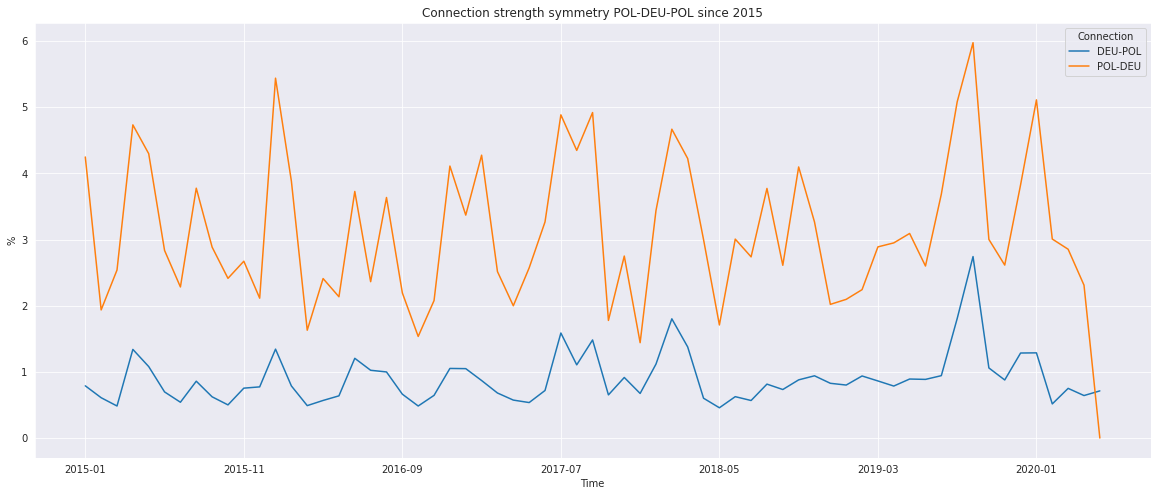
\includegraphics[width=\linewidth]{fig/POL-DEU-POL.png}
        \caption{Symetryczność siły połączenia Polski i~Niemiec w~czasie. (źródło: opracowanie własne)}
        \label{fig:POL-DEU-POL}
    \end{figure}


    Wykres~\ref{fig:POL-RUS-POL} przedstawia symetryczność siły połączenia Polski i~Rosji w~czasie.
    \begin{figure}[!htp]
        \centering
        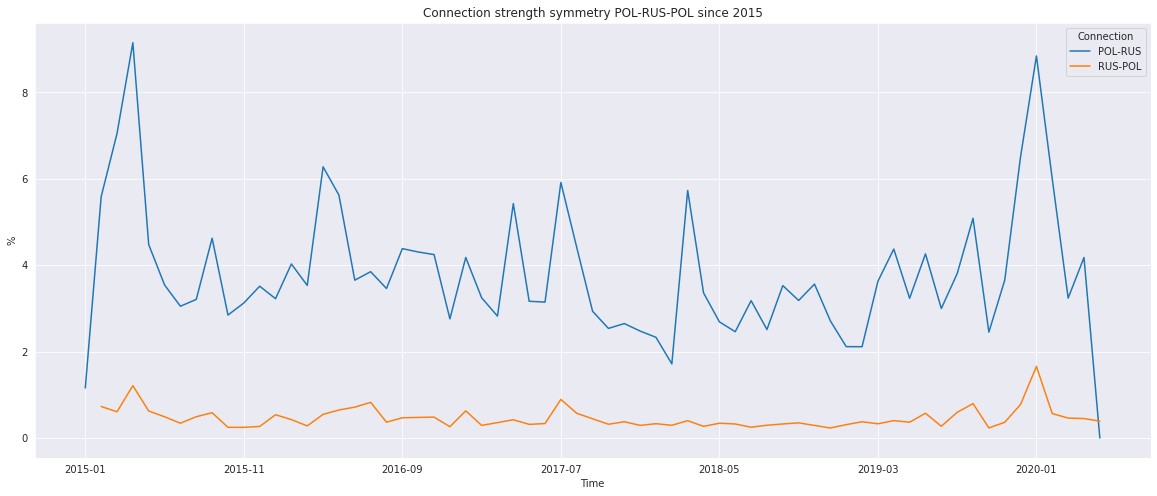
\includegraphics[width=\linewidth]{fig/POL-RUS-POL.png}
        \caption{Symetryczność siły połączenia Polski i~Rosji w~czasie. (źródło: opracowanie własne)}
        \label{fig:POL-RUS-POL}
    \end{figure}


    \chapter{Realizacja}\label{ch:realizacja}


    \section{Wybór systemu agentowego}

    W języku Python istnieje wiele bibliotek do analizy danych oraz uczenia maszynowego.
    Aby uniknąć potrzeby generowania powiązań z innymi językami platforma agentowa będzie również w Pythonie.
    Poniżej przeanalizowano zalety i wady kilku wybranych platform w tym języku.

    \begin{table}[]
        \begin{tabular}{l|ll}
            & SPADE                                   & PADE                     \\ \hline
            komunikacja            & serwer XMPP                             & biblioteka Twisted       \\
            & FIPA, XMPP Data Forms~\cite{data_forms} & FIPA ACL~\cite{fipa_acl} \\ \hline
            filtrowanie wiadomości & metadane                                & klasa filtrująca         \\ \hline
            licencja               & MIT                                     & MIT                      \\ \hline
            transfer               & zserializowani agenci                   & agenci mogą być          \\
            &                                         & zawartością wiadomości   \\ \hline
            zachowania             & wiele jednocześnie:                     & cykliczne i periodyczne  \\
            & cykliczne i periodyczne \\ \hline
            obecność kontaktów     & powiadomienia                           & -                        \\
            & w czasie rzeczywistym \\ \hline
            interfejs graficzny    & webowy                                  & webowy (Flask)           \\ \hline
            rozszerzenia           & wtyczki                                 & -                        \\ \hline \hline
        \end{tabular}
        \caption{Porównanie wybranych platform wieloagentowych w języku python. (źródło: opracowanie własne)}
        \label{tab:porownanie}
    \end{table}

    \subsection{Mesa}
    Mesa~\cite{Masad2015} to biblioteka do modelowania agentowego w Pythonie.
    Pozwala na szybkie stworzenie modelu agentowego przy wykorzystaniu wbudowanych komponentów.
    \href{https://github.com/projectmesa/mesa}{Project~Mesa~github}
    Ostatnie zmiany na githubie 11 lutego 2021 (stan na 17 II 2021r.).

    \subsection{Python Agent DEvelopment framework}
    Framework PADE~\cite{Melo2019} umożliwia rozwój, wykonanie i zarządzanie wieloagentowymi systemami w rozproszonym środowisku.
    \href{https://github.com/grei-ufc/pade}{Smart~Grids~Research~Group~-~UFC~github}
    Ostatnie zmiany na githubie 4 lutego 2021 (stan na 17 II 2021r.).

    \subsection{Smart Python multi-Agent Development Environment}
    Platforma wieloagentowa SPADE jest oparta o XMPP\cite{Saint-Andre2007}.
    \href{https://github.com/javipalanca/spade}{javipalanca~github}
    Ostatnie zmiany na githubie 22 maja 2020 (stan na 17 II 2021r.).


    \chapter{Ewaluacja}\label{ch:ewaluacja}


    \chapter{Podsumowanie}\label{ch:podsumowanie}

    \appendix
    \newpage


    \chapter{Instalacja platformy wieloagentowej}


    \section{Prosody}
    Do działania platformy SPADE niezbędny jest serwer XMPP.
    Przykładem takiego oprogramowania na licencji otwarto-źródłowej jest Prosody.
    Prosody~\cite{prosody} jest nowoczesnym serwerem komunikacyjnym XMPP.
    W celu jego instalacji w systemie operacyjnym Linux Debian lub Ubuntu należy skorzystać z polecenia:
    \begin{verbatim}
           sudo apt-get install prosody
    \end{verbatim}

    Dodanie użytkownika następuje przez wydanie polecenia:
    \begin{verbatim}
        sudo prosodyctl adduser me@localhost
    \end{verbatim}

    Aby zezwolić użytkownikom na rejestrację nowych kont i zmianę haseł należy edytować plik:
    \begin{verbatim}
        /etc/prosody/prosody.cfg.lua
    \end{verbatim}
    zmieniając na: \textit{allow\_registration = true;}
    Następnie należy zrestartować program Prosody używając polecenia:
    \begin{verbatim}
        sudo /etc/init.d/prosody restart
    \end{verbatim}.


    \section{SPADE}

    Aby zainstalować SPADE wystarczy w terminalu wydać polecenie:
    \begin{verbatim}
        pip install spade
    \end{verbatim}

    W celu stworzenia agenta należy postępować wg instrukcji~\cite{SPADEquickstart}:
    \begin{verbatim}
    from spade import agent

    class DummyAgent(agent.Agent):
        async def setup(self):
            print("Hello World! I'm agent {}".format(str(self.jid)))

    dummy = DummyAgent("your_jid@your_xmpp_server", "your_password")
    dummy.start()

    dummy.stop()
    \end{verbatim}

    W SPADE do tworzenia wiadomości przeznaczona jest klasa \textit{Message},
    która pozwala na wprowadzenie metadanych do wiadomości.
    Metadane w postaci słowników klucz, wartość są przydatne do uwzględnienia atrybutów FIPA.

    Funkcje \textbf{send} oraz \textbf{receive} są procesami asynchronicznymi dlatego należy je wywoływać z instrukcją \textit{await}.
    Ponieważ SPADE jest platformą do przesyłania wiadomości w czasie rzeczywistym,
    to wysłana wiadomość przepadnie jeśli odbiorca nie jest gotowy na jej odebranie.
    Dzięki XMPP agenci SPADE są zdolni do utrzymywania listy kontaktów i mogą otrzymywać powiadomienia o ich kontaktach w czasie rzeczywistym.
    Ta funkcjonalność pozwala podnieść niezawodność komunikacji.


    \section{BigQuery}
    W celu zainstalowania biblioteki google cloud dla języka python należy skorzystać z polecenia:
    \begin{verbatim}
        pip install --upgrade 'google-cloud-bigquery[bqstorage,pandas]'
    \end{verbatim}


    \section{fpdf2}
    fpdf2 to minimalistyczna bilblioteka do tworzenia plików PDF w Python.
    W celu zainstalowania bilbioteki fpdf2 należy skorzystać z polecenia:
    \begin{verbatim}
        pip install fpdf2
    \end{verbatim}


    \chapter{table en}

    \begin{table}[ht!]
        \begin{tabular}{ll}
            Role schema:             & Correlation Seeker                                          \\ \hline
            Description              & This role includes finding correlations between countries   \\
            & based on data collected from Pattern Seekers.               \\
            Protocols and Activities & \textbf{checkPatterns, searchForCorrelation, tellGenerator} \\
            Permissions              & \textbf{reads delivered} \textit{PatternSeeker}             \\
            & ~~~~~~\textit{pattern}                                      \\
            & \textbf{change} \textit{statement}                          \\
            Responsibilities         &                                                             \\
            ~~vitality               & \textbf{checkPatterns, searchForCorrelation, tellGenerator} \\
            ~~security               & -                                                           \\
        \end{tabular}
        \caption{Correlation Seeker role schema. (source: own research)}
    \end{table}

    \begin{table}[ht!]
        \begin{tabular}{ll}
            Role schema:             & Comparison Generator                                               \\ \hline
            Description              & This role includes creating comparisons from                       \\
            & data collected by Correlation and Trend Seekers.                   \\
            Protocols and Activities & \textbf{checkComparisons}                                          \\
            Permissions              & \textbf{reads delivered} \textit{Correlation Seeker, Trend Seeker} \\
            & ~~~~~~\textit{comparison}                                          \\
            & \textbf{change} \textit{comparison}                                \\
            Responsibilities         &                                                                    \\
            ~~vitality               & \textbf{checkComparison}                                           \\
            ~~security               & -                                                                  \\
        \end{tabular}
        \caption{Comparison Generator role schema. (source: own research)}
    \end{table}

    \begin{table}[ht!]
        \begin{tabular}{ll}
            Role schema:             & Pattern Seeker                              \\ \hline
            Description              & This role includes pattern searching        \\
            & among the data using a set of measures.     \\
            & Patterns fall into two categories: internal \\
            & and between countries.                      \\
            Protocols and Activities & \textbf{SearchPatterns}                     \\
            Permissions              & \textbf{reads} \textit{measures}            \\
            & \textbf{change} \textit{pattern}            \\
            Responsibilities         &                                             \\
            ~~vitality               & \textbf{SearchPatterns}                     \\
            ~~security               & -                                           \\
        \end{tabular}
        \caption{Pattern Seeker role schema. (source: own research)}
    \end{table}


    \chapter{Prototyp v1}
    System agentowy składający się z:
    \begin{itemize}
        \item jednego agenta Generator Zestawień
        \item jednego agenta Poszukiwacza Trendów
%        todo sprawdź czy rzeczywiście 30 kombinacji
        \item 30 agentów Poszukiwacz Wzorców - po jednym dla każdej kombinacji państw.
    \end{itemize}

    Generator Zestawień tworzy agenta Poszukiwacz Trendów.
    Agent Poszukiwacz Trendów tworzy dla każdej pary krajów Poszukiwacza Wzorców.
    Poszukiwacz Wzorców sprawdza symetrię/asymetrię relacji~\ref{symetria_relacji} pomiędzy parą krajów badając siłę powiązania miedzy nimi, w kolejnych okresach czasu.
    Wyniki są zwracane do Poszukiwacza Trendów który analizuje zebrane dane szukając tendencji.
    Ostateczne wyniki przekazywane są do Generatora Zestawień który przygotowuje raport końcowy.

    \paragraph{Symetria relacji}
    \[ Percentage = \frac
    {\sum{Events\ country\ A\ (actor 1)\ with\ Country\ B\ (actor 2)}}
    {\sum{Events\ country\ A\ (actor 1)}}
    \]

    \paragraph{Wzorzec Mocarstwo/Klient}

    \subparagraph{Relacje istotne}
%    todo przeredagować
    Wg pracy Jarosza.
    Relacje znaczące to takie wydarzenia które posiadają co najmniej 50 wzmianek w mediach (NumMentions)//s. 33.

    Wzorzec Mocarstwo/Klient określony jako stosunek liczby wszystkich relacji znaczących Aktora 1 oraz liczby wszystkich znaczących relacji Aktora2 //s. 82.
    \[ Ratio = \frac
    {\sum{Events\ country\ A\ (actor 1) (NumMentions > 50)}}
    {\sum{Events\ country\ B\ (actor 1) (NumMentions > 50)}}
    \]

    \paragraph{Kraje do testów}
    \begin{enumerate}
        \item Polska
        \item Niemcy
        \item Rosja
        \item Czechy
        \item Słowacja
        \item Ukraina
    \end{enumerate}
    6 krajów - 30 kombinacji

    Zakres czasu jaki powinien być analizowany jest przekazywany z Generatora Zestawień.
    Analizowane zostaną wszystkie kraje (z puli testowej)lub te wybrane przez Generator.
    Analizowany jest tylko wzorzec symetria/asymetria.
    Początkowo analiza prowadzona jest w miesięcznych przedziałach czasu.
    Jeśli wyniki będą bardzo zaburzone, zwiększone zostaną analizowane przedziały czasu.
    Jeśli wyniki będą stałe możliwe będzie przejście na mniejsze przedziały.
    Diagram czynności prototypu został przedstawiony na rysunku~\ref{fig:diagram_czynności_top}.
    Diagram czynności przedstawia logikę algorytmu w postaci sekwencji aktywności.
    Upraszcza i ulepsza proces dzięki wyjaśnieniu skomplikowanych przypadków.

    \begin{figure}[!ht]
        \centering
        \includegraphics[width=\linewidth]{fig/diagrams/Diagram czynności top ALL.pdf}
        \caption{Diagram czynności systemu. (źródło: opracowanie własne)}
        \label{fig:diagram_czynności_top}
    \end{figure}


    \section{Parametry konfiguracyjne}
    Parametry konfiguracyjne mogą być podawane na wejście systemu.
    Część parametrów może być określana w postaci przedziałów, z których system wybierze wartości.
    Niektóre z parametrów mogą być dobierane w pełni automatycznie na zasadzie uczenia maszynowego.
%    Manualne, pół-automatyczne, automatyczne.

    \subsection{Tylko wybrane kraje}
    Lista krajów które będą analizowane jako jedyne.

    \subsection{Kraje szczególnego zainteresowania}
    Lista krajów dla których system będzie starał się znaleźć najwięcej informacji.

    \subsection{Zdarzenia szczególnego zainteresowania}
    Podane w formie dat główne punkty w pobliżu których system powinien przeprowadzać poszukiwania.

    \subsection{Wielkość okna czasowego}
    Rozmiar przedziałów czasu w jakich agregowane będą analizowane dane.
    Poziomy granulacji czasu:
    \begin{itemize}
        \item tydzień,
        \item miesiąc,
        \item rok.
    \end{itemize}
    Okno czasowe może być zmieniane przez system wg.~\ref{subsec:przedziały-czasowe}.

    \subsection{Punkt stopu poszukiwań}
%    W którym momencie który agent powinien zaprzestawać dalszej analizy?
    Cyklicznie sprawdzane warunki pozwalające określić czy dalsze przeszukiwanie jest zasadne.

    \subsection{Data początku i końca analizy}
    Przedział czasu określający badany przez system okres.

    \subsection{Progi dla danego kraju/relacji}\label{subsec:progi-dla-danego-kraju/relacji}
    Progi pozwolą na odrzucenie poszukiwań w mało interesujących obszarach.
    Mogą być dobierane ręcznie, pół-automatycznie, lub automatycznie.
    Możliwe do wyboru progi:
    \begin{itemize}
        \item liczba zdarzeń (pokazuje aktywność podmiotów z danego kraju - ZAKRES),
        \item liczba wzmianek (pokazuje, że dane działanie było uznane za ważne - WAGA),
        \item liczba źródeł,
        \item średni średni ton,
        \item miara Goldsteina
        \item stosunek liczby zdarzeń (pokazuje jak nastawione jest dane państwo).
        \item liczba silnych relacji kooperacyjnych,
        \item liczba silnych relacji wrogich.
    \end{itemize}

    \subsection{Podpowiedź prawdopodobnego wyniku}\label{subsec:podpowiedź-prawdopodobnego-wyniku}
    Podpowiedzi dla systemu pochodzące z pliku konfiguracyjnego.
    W celu poprawy weryfikacji podpowiadane są prawdopodobne wyniki jakie chcemy otrzymać,
    np.: Izrael - Iran -> wrogowie, USA - Polska -> mocarstwo - klient.

    \subsection{Zadane algorytmy klastrowania}
    Możliwe do wyboru algorytmy klastrowania:
    \begin{itemize}
        \item k-means
        \item aglomeracyjne
        \item DBSCAN
    \end{itemize}


    \section{Miary i wzorce}
    Miar zostały opisane w sekcji~\ref{sec:miary}.
    Wzorce zostały opisane w sekcji~\ref{sec:wybór-wzorców}


    \section{Otwarte problemy}

    \subsection{Klastrowanie}
    Gdzie odbędzie się klastrowanie?
    Wg jakich miar?

    \subsubsection{Klastrowanie państw}
    Łączenie podobnych państw w grupy na podstawie wybranych miar.
    Wyodrębnienie państw:
    \begin{itemize}
        \item silnych,
        \item bogatych,
        \item aktywnych politycznie
        \item związanych z przemocą
        \item o wyraźnie podwyższonych nakładach na opiekę zdrowotną / zbrojenia
        \item \ldots
    \end{itemize}

    \paragraph{Przykład}

    Grupowanie państw w~klastry z wykorzystaniem wektora cech z~bazy GDELT oraz algorytmu klastrowania k-średnich.
    Wektor danych dla każdego kraju składa się z:
    \begin{enumerate}
        \item[•] liczby zdarzeń w~analizowanym okresie, w~których dany kraj jest aktorem 1,
        \item[•] sumy liczby wzmianek (całkowitej liczby wzmianek o~tym wydarzeniu, we wszystkich dokumentach źródłowych podczas 15-minutowej aktualizacji, w~której zostało po raz pierwszy zauważone) w~analizowanym okresie, dla wydarzeń w~których dany kraj jest aktorem 1,
        \item[•] stosunku liczby zdarzeń w~analizowanym okresie, w~których dany kraj jest aktorem 1, oznaczonych \textit{quad class} jako \textit{material conflict} do liczby zdarzeń w~analizowanym okresie, w~których dany kraj jest aktorem 1, oznaczonych \textit{quad class} jako \textit{material cooperation},
        \item[•] stosunku liczby zdarzeń w~analizowanym okresie, w~których dany kraj jest aktorem 1, oznaczonych \textit{quad class} jako \textit{verbal conflict} do liczby zdarzeń w~analizowanym okresie, w~których dany kraj jest aktorem 1, oznaczonych \textit{quad class} jako \textit{verbal cooperation},
        \item[•] średniego, dla wszystkich zdarzeń w~analizowanym okresie, w~których dany kraj jest aktorem 1, średniego tonu (średni „ton” wszystkich dokumentów zawierających jedną lub więcej wzmianek o~tym wydarzeniu, podczas 15-minutowej aktualizacji, w~której zostało ono po raz pierwszy zauważone, waha się od -100 (skrajnie ujemny) do +100 (skrajnie dodatni)),
        \item[•] średniej, dla wszystkich zdarzeń w~analizowanym okresie, w~których dany kraj jest aktorem 1, miary Goldsteina (skala Goldsteina przypisuje wynik liczbowy od -10 do +10, wychwytując teoretyczny potencjalny wpływ, jaki rodzaj zdarzenia będzie miał na stabilność kraju),
        \item[•] liczby zdarzeń w~analizowanym okresie, w~których dany kraj jest aktorem 1, oznaczonych \textit{event root code} jako \textit{fight} Fight,
        \item[•] liczby zdarzeń w~analizowanym okresie, w~których dany kraj jest aktorem 1, oznaczonych \textit{event root code} jako \textit{Express intent to cooperate}.
    \end{enumerate}
    Wykorzystane dane pochodzą ze stycznia 2020 roku.
    Przed dokonaniem klasteryzacji odrzucone zostały wydarzenia z~kodami krajów cameo niezgodnymi z~kodami ISO 3166-1 alfa-3~\cite{iso_alfa3}.

    Wykres~\ref{fig:clust10std} przedstawia mapę z~naniesionymi wynikami klasteryzacji ustandaryzowanych próbek.
    Każda grupa krajów otrzymała inny kolor.
    Zauważalne są skupiska geograficzne krajów należących do danego klastra.

    \begin{figure}[!htp]
        \centering
        \includegraphics[width=\linewidth]{fig/pp/10clusterMap_std.png}
        \caption{Mapa z~wynikami klasteryzacji. (źródło: opracowanie własne)}
        \label{fig:clust10std}
    \end{figure}

    \subsubsection{Klastrowanie relacji}
    Łączenie podobnych relacji w grupy na podstawie wybranych miar.
    Wyodrębnienie relacji:
    \begin{itemize}
        \item mocarstwo - klient
        \item sojusznicy
        \item wrogowie
        \item symetria/asymetria
    \end{itemize}

    \subsubsection{Klastrowanie w czasie}
    Jak zmienia się przynależność kraju do klastrów?
    Zmiana/oscylacja/piki.

    \paragraph{Korelacja}
    Jaki współczynnik korelacji(Pearsona?)?
    \begin{itemize}
        \item zmiany następują z opóźnieniem,
        \item zmiany następują jednocześnie,
        \item jak często (procentowo) trafiają do tego samego klastra,
        \item jak często (procentowo) trafiają do różnych klastrów ale zmiana zachodzi w tym samym czasie.
        Dynamika relacji.
        Uchwycenie podobieństwa w zachowaniu.
        Powiązanie zmiany relacji (np.: sojusznik ->wróg) z wydarzeniami.
        \item procentowa (w czasie) przynależność do tego samego,
        \item jak często zmiana klastra przez oba państwa występuje w tych samych tygodniach.
        \item korelacja miedzy miarami, a stanem gospodarczym
        \item powiązanie zmiany relacji z wydarzeniami
        \item powiązanie z kursem giełdowym?
    \end{itemize}

    \subsection{Porównanie państw}
    Porównywanie wybranych państw.

    \subsection{Porównywanie relacji}
    Porównywanie wybranych relacji.

    \subsection{Ważne wydarzenia}
    Daty ważnych wydarzeń podawane w formie pliku na wejście jako punkt zaczepienia do poszukiwań w koło tej daty.

    \subsection{Rodzaje przeszukiwania - zmienność/agregacja}
    Agregacja gdy pojawia się stały poziom.
    Preferencja rodzaju przeszukiwania podana w konfiguracji.

    \subsection{Przedziały czasowe}\label{subsec:przedziały-czasowe}
    Jeśli są mocne zmiany zachowań dla szerokiego przedziału, zmniejsz przedział aby uniknąć lokalnych fluktuacji.
    Jeśli jest stała wartość dla relacji to zacznij badać dla mniejszego przedziału.

    \subsection{Agregacja}
    Poszukiwacz wzorców może mieć miarę zagregowaną na różnych poziomach.

    \subsection{Badanie relacji odwrotnej}
    Dla tej samej relacji zamieniamy Aktora 1 i Aktora 2.
    W niektórych przypadkach może to stanowić redundancję która ułatwi dalsze obliczenia.

    \subsection{Mało zdarzeń - informacja dodatkowa}
    Zwracanie dodatkowej informacji do poszukiwacza o tym, że analizowanych wydarzeń jest mało.

    \subsubsection{Zaprzestanie poszukiwań}
    Poszukiwacz trendów może decydować o zaprzestaniu poszukiwania relacji gdy zdarzeń jest zbyt mało.

    \subsection{Dużo zdarzeń - informacja dodatkowa}
    Zwracanie dodatkowej informacji do poszukiwacza o tym, że analizowanych wydarzeń jest dużo.

    \subsubsection{Histogram}
    Generowanie dodatkowego histogramu gdy danych zdarzeń jest bardzo dużo.

    \subsubsection{Uruchomienie poszukiwań korelacji}
    Ewentualne uruchomienie poszukiwań korelacji gdy zdarzeń jest bardzo dużo.

    \subsection{Inteligentna selekcja wyników}
    Selekcja wyników będzie podstawą do dalszej eksploracji.

    \subsection{Kraje szczególnego zainteresowania}
    Wskazanie w konfiguracji jakie kraje są szczególnie interesujące.

    \subsection{Podpowiedzi konfiguracyjne}\label{subsec:podpowiedzi-konfiguracyjne}
    Realizacja punktu~\ref{subsec:podpowiedź-prawdopodobnego-wyniku}.

    \subsection{Reset systemu w przypadku niezadowalającej odpowiedzi}
    Reset systemu z nowymi parametrami.

    \subsection{Komunikacja z agentami wyższego rzędu tylko w przypadku znalezienia istotnych informacji}

    \subsection{Filtrowanie relacji/krajów na podstawie wartości progowej}
    Relacje krajów europejskich z krajami azjatyckimi mają małe znaczenie i powinny zostać odfiltrowane.
    Progi - patrz~\ref{subsec:progi-dla-danego-kraju/relacji}.

    \subsection{Wykorzystanie analogii}
    Coś ciekawego w jednym państwie/relacji może być wskazówką do poszukiwania w drugim/drugiej.

    \subsection{Poszukiwacz Wzorców Wewnętrznych}
    Dedykowany agent zajmujący się poszukiwaniem wzorców wewnątrz kraju.
    Agent związany z krajem może wstępnie badać relacje z innymi krajami
    i powołać agenta który będzie odpowiadał za badanie tych relacji.
    Takie działanie pozwoli ograniczyć liczbę badanych relacji, odrzucić relacje niepożądane.

    \subsection{Jak sojusznicy USA reagują na pogorszenie relacji danego państwa ze Stanami?}

    \subsection{Jakie eksperymenty? Co w nich zebrać? Czego system ma się uczyć?}
    granulacja, korelacja, średnie, zakresy czasowe

    \subsection{Pytania badawcze}
    \begin{itemize}
        \item Znajdź kraje z którymi dany kraj jest w dobrych/złych relacjach.
        \item Znajdź relacje podobne do relacji POL-RUS (jakie relacje są najbardziej podobne) /relacja POL-RUS opisana zestawem miar/
        /czy system znajdzie coś zgodnego z intuicją czy raczej coś dziwnego/
        \item Jak Czechy są postrzegane w relacji z Polską?
        \item Kto jest hegemonem dla Polski na podstawie miar lub podobieństwo do relacji POL-USA.
    \end{itemize}

    \subsection{Sterowanie w oparciu o jaka miarę?}
    prawdopodobieństwo (determinizm)
    wyszukiwanie z listą tabu
    losowanie konfiguracji (może uczenie genetyczne)

    \subsection{Identyfikacja relacji wrogich}
    Czy są stabilne?
    Przewidywanie dalszego przebiegu relacji.

    \subsection{Identyfikacja przynależności do klastrów w czasie}
    Czy kraj trafia ciągle do tego samego klastra?
    - stabilność, oscylacja, pojedyńcza zmiana z A do B, pojedyńcze zaburzenie ABA

    \subsection{Poszukiwanie przejśc ABA w relacjach}
    W jaki terminie się znajdują.

    \subsection{Po automatycznym policzeniu miar -> klastrowanie}
    \begin{itemize}
        \item Jak klastry są odseparowane?
        \item Które miary dobrze separują z punktu widzenia celu?
        System może podpowiadać na jakie miary warto zmieniać wna podstawie miary jakości kastrowania (patrz literatura).
        Które klastrowanie jest najlepsze z punktu widzenia separowalności (ciężko zaliczyć element z jednego klastra do innego w oparciu o miarę).
        Wiemy które kraje powinny być we wspólnym klastrze -> chcemy dobrać miary.

        \item Na ile udało się dobrze dobrać klastry?
        np.: relacje przyjazne/wrogie w jednym klastrze
        państwa o podobnym potencjale
        podobny potencjał militarny
        podobny potencjał militarny i duże wydatki na opiekę zdrowotną
        duże PKB (różne klasy w oparciu o klastry)

        \item Kiedy kraje trafiają do tych samych kategorii?
        Czy mamy zmienność przynależności w czasie?
        Które relacje sa stabilne?
    \end{itemize}

    \subsection{Badanie dynamiki}

    \subsection{Podobieństwo statyczne}

    \subsection{Podobieństwo zagregowane}


    \section{Działające elementy systemu}
    \begin{itemize}
        \item Raportowanie PDF
        \begin{itemize}
            \item analiza symetrii
            \item Power-Client
            \item Pairwise correlation
        \end{itemize}
        \item Bez raportu
        \begin{itemize}
            \item cooperate
            \item cooperate mentions >=5 >=10
            \item fight
            \item correlation
            \begin{itemize}
                \item Spearman
                \item Pearson
                \item Kendall
            \end{itemize}
            \item autocorrelation
            \item crosscorrelation
            \item rolling median
            \item symmetry 1 2 3 4 5 6 12 M
        \end{itemize}
    \end{itemize}


    \section{Analiza zdarzeń wewnętrznych USA}
    W tym dodatku przedstawiona została analiza zdarzeń wewnętrznych w Stanach Zjednoczonych.

    \subsection{Kody bazowe (Event Base Codes)}
    W tej części zastały porównane liczby kodów bazowych.

    Wykres~\ref{fig:USA_inner_EBC} przedstawia liczbę liczbę zdarzeń wewnętrznych w USA z poszczególnymi kodami bazowymi.
    Wykres~\ref{fig:USA_inner_EBCperc} przedstawiają procentowy udział zdarzeń wewnętrznych w USA z poszczególnymi kodami bazowymi.

    \begin{figure}[!htp]
        \centering
        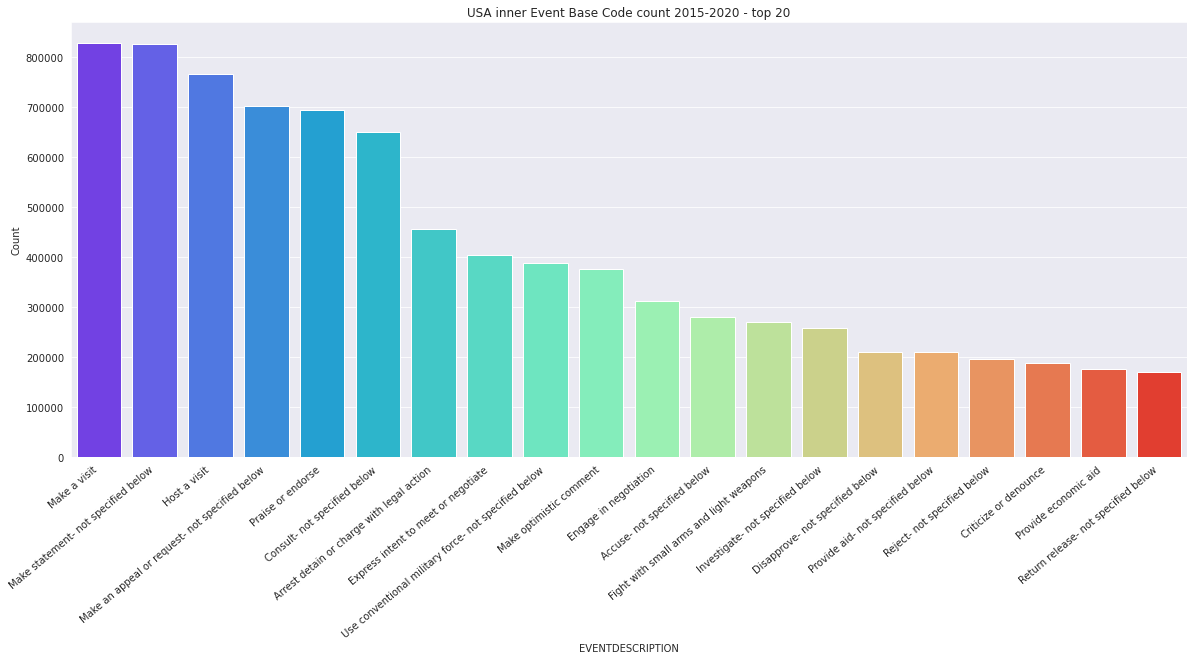
\includegraphics[width=\linewidth]{fig/USA inner/EBC.png}
        \caption{Liczba zdarzeń wewnętrznych USA dla kodów bazowych od 2015 - top 20. (źródło: opracowanie własne)}
        \label{fig:USA_inner_EBC}
    \end{figure}

    \begin{figure}[!htp]
        \centering
        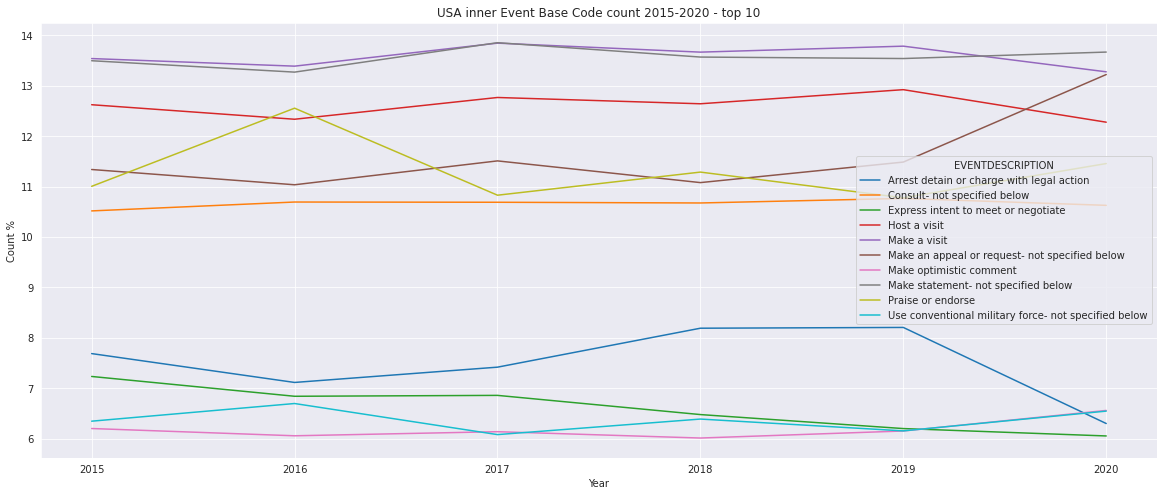
\includegraphics[width=\linewidth]{fig/USA inner/EBCperc.png}
        \caption{Procentowa liczba zdarzeń wewnętrznych USA dla kodów bazowych od 2015 - top 10. (źródło: opracowanie własne)}
        \label{fig:USA_inner_EBCperc}
    \end{figure}

    Wykres~\ref{fig:USA_not_inner_EBC} przedstawia liczbę liczbę zdarzeń pomiędzy USA i innymi krajami z poszczególnymi kodami bazowymi.
    Wykres~\ref{fig:USA_not_inner_EBCperc} przedstawiają procentowy udział zdarzeń pomiędzy USA i innymi krajami z poszczególnymi kodami bazowymi.

    \begin{figure}[!htp]
        \centering
        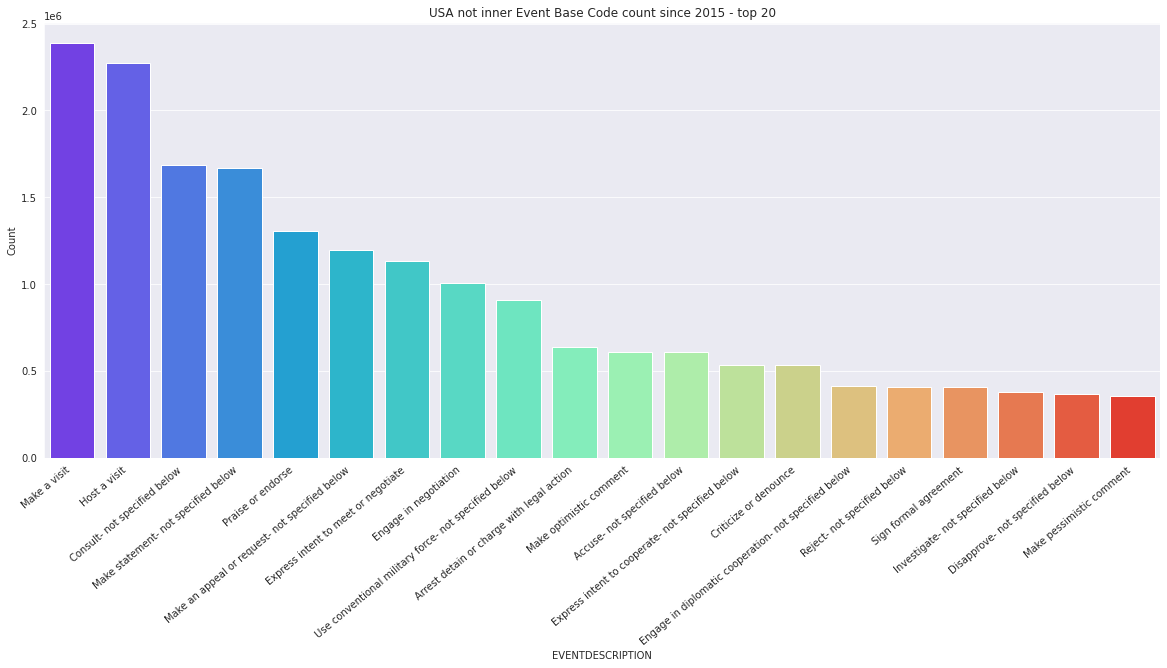
\includegraphics[width=\linewidth]{fig/USA not inner/EBC.png}
        \caption{Liczba zdarzeń zewnętrznych USA dla kodów bazowych od 2015 - top 20. (źródło: opracowanie własne)}
        \label{fig:USA_not_inner_EBC}
    \end{figure}

    \begin{figure}[!htp]
        \centering
        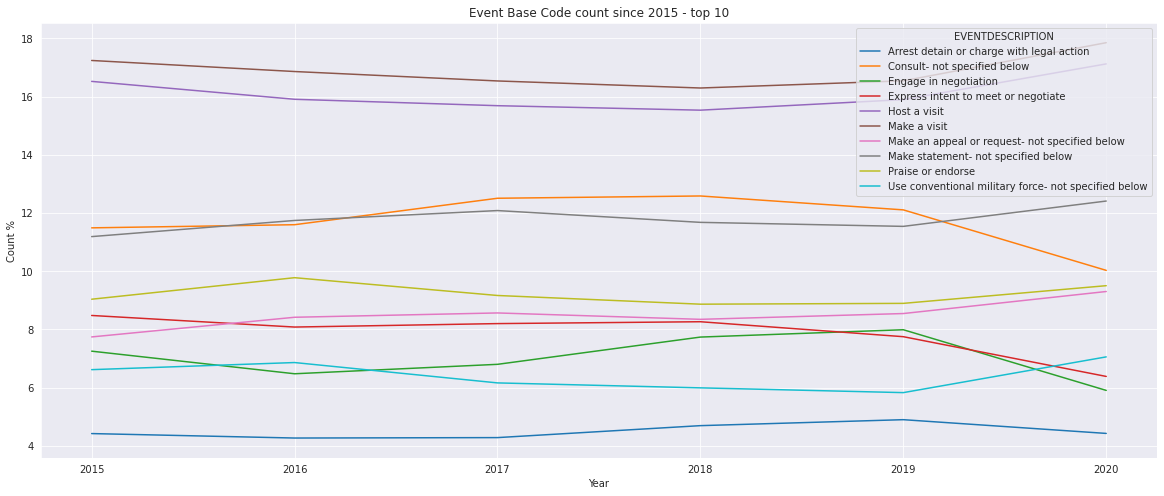
\includegraphics[width=\linewidth]{fig/USA not inner/EBCperc.png}
        \caption{Procentowa liczba zdarzeń zewnętrznych USA dla kodów bazowych od 2015 - top 10. (źródło: opracowanie własne)}
        \label{fig:USA_not_inner_EBCperc}
    \end{figure}

    Wykres~\ref{fig:GLOBAL_EBC} przedstawia globalną liczbę liczbę zdarzeń z poszczególnymi kodami bazowymi.
    Wykres~\ref{fig:GLOBAL_EBCperc} przedstawiają globalny procentowy udział zdarzeń z poszczególnymi kodami bazowymi.

    \begin{figure}[!htp]
        \centering
        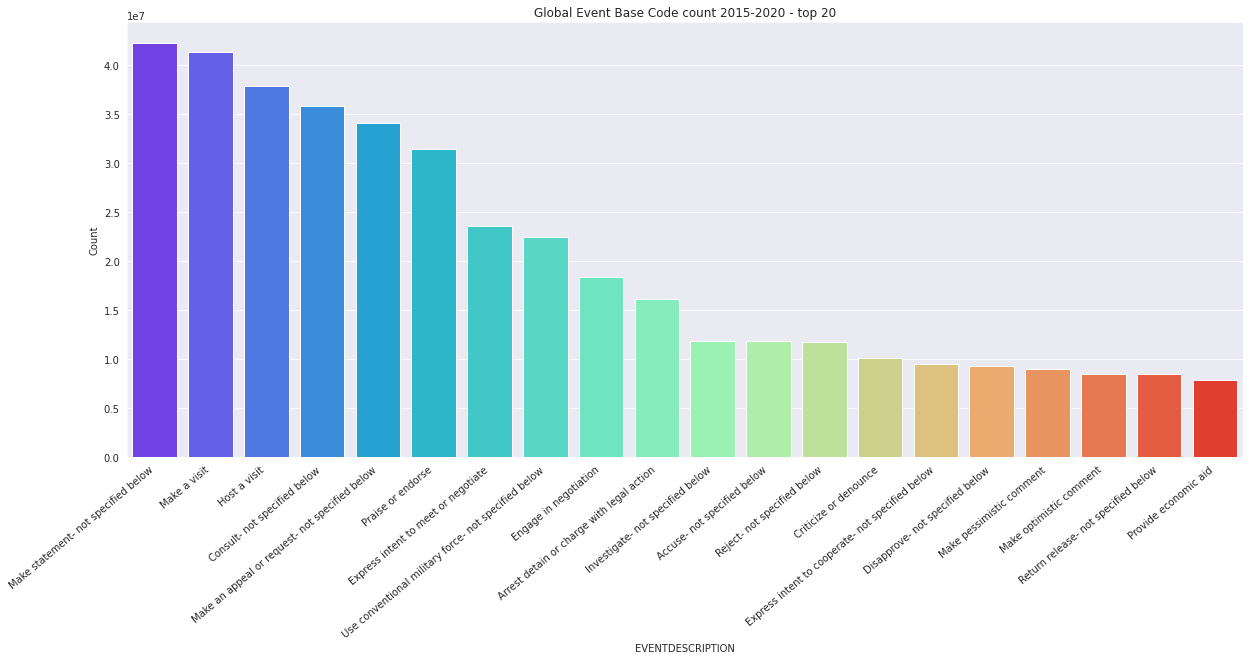
\includegraphics[width=\linewidth]{fig/GLOBAL//EBC.png}
        \caption{Liczba zdarzeń dla kodów bazowych od 2015 - top 20. (źródło: opracowanie własne)}
        \label{fig:GLOBAL_EBC}
    \end{figure}

    \begin{figure}[!htp]
        \centering
        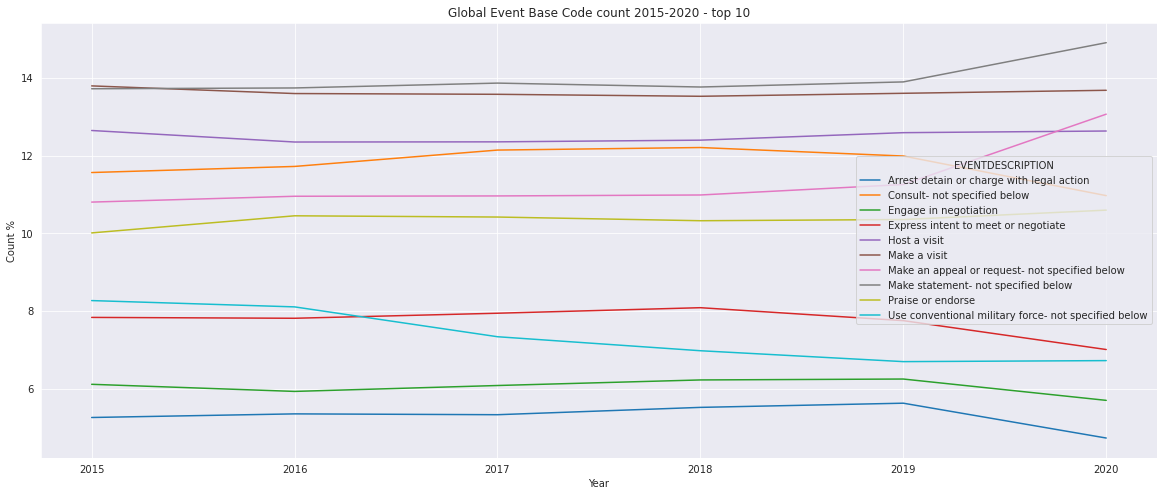
\includegraphics[width=\linewidth]{fig/GLOBAL//EBCperc.png}
        \caption{Procentowa liczba zdarzeń dla kodów bazowych od 2015 - top 10. (źródło: opracowanie własne)}
        \label{fig:GLOBAL_EBCperc}
    \end{figure}

    Liczba zdarzeń wewnętrznych \textit{Make a visit} w USA w latach 2015-2020 to około 810 tysięcy.
    Zdarzeń zewnętrznych \textit{Make a visit} w USA w tym okresie było 3 razy więcej - około 2,4 miliona,
    podczas gdy globalna liczba zdarzeń \textit{Make a visit} wynosiła około 41 milionów.

    Zarówno dla zdarzeń wewnętrznych USA, jak i globalnych w pierwszej trójce występują zdarzenia:
    \begin{itemize}
        \item \textit{Make a visit},
        \item \textit{Make statement - not specific below},
        \item \textit{Host a visit}.
    \end{itemize}
    Dla zdarzeń zewnętrznych USA w pierwszej trójce \textit{Make statement - not specific below} zostaje zastąpione przez \textit{Consult - not specific below}.
    \textit{Make statement - not specific below} pojawia się na 4 pozycji.

    Takie wyniki mogą świadczyć o podobieństwie klasyfikacji bazowej (Base Codes) zdarzeń,
    niezależnie od tego czy są to zdarzenia wewnętrzne czy zewnętrzne.

    \subsection{Kody podstawowe (Event Root Codes)}

    Wykres~\ref{fig:USA_inner_ERC} przedstawia liczbę zdarzeń wewnętrznych w USA z poszczególnymi kodami podstawowymi.
    Wykres~\ref{fig:USA_inner_ERCperc} przedstawiają procentowy udział zdarzeń wewnętrznych w USA z poszczególnymi kodami podstawowymi.


    \begin{figure}[!htp]
        \centering
        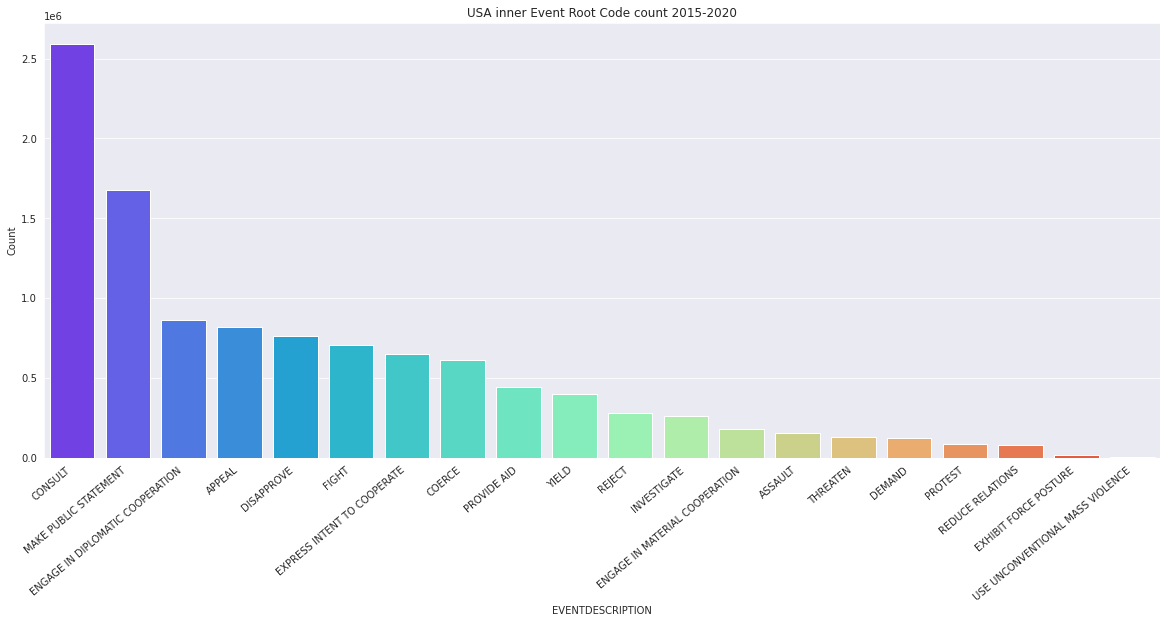
\includegraphics[width=\linewidth]{fig/USA inner/ERC.png}
        \caption{Liczba zdarzeń wewnętrznych USA dla wszystkich kodów podstawowych od 2015. (źródło: opracowanie własne)}
        \label{fig:USA_inner_ERC}
    \end{figure}

    \begin{figure}[!htp]
        \centering
        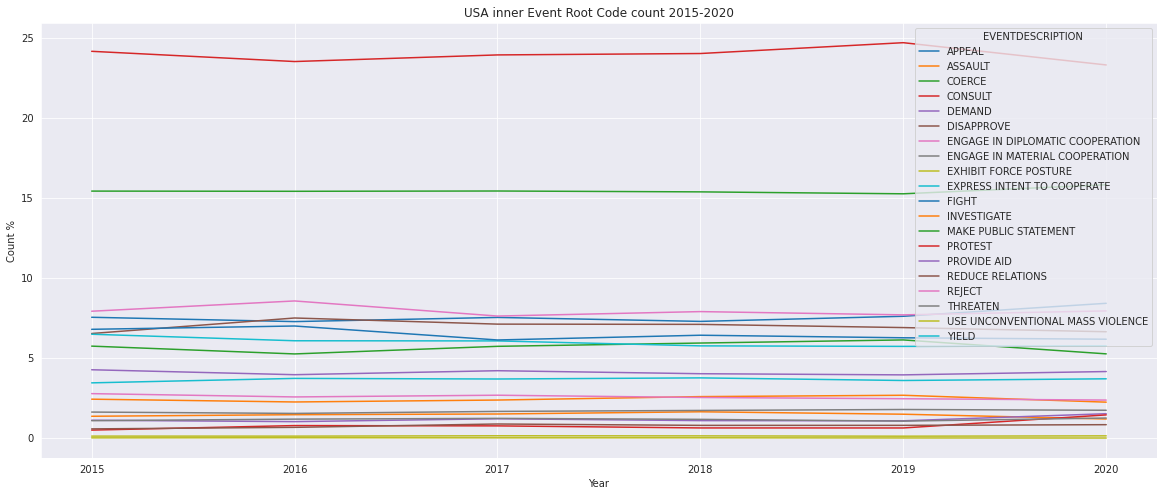
\includegraphics[width=\linewidth]{fig/USA inner/ERCperc.png}
        \caption{Procentowa liczba zdarzeń wewnętrznych USA dla wszystkich kodów podstawowych od 2015. (źródło: opracowanie własne)}
        \label{fig:USA_inner_ERCperc}
    \end{figure}

    Wykres~\ref{fig:USA_not_inner_ERC} przedstawia liczbę zdarzeń pomiędzy USA i innymi krajami z poszczególnymi kodami podstawowymi.
    Wykres~\ref{fig:USA_not_inner_ERCperc} przedstawiają procentowy udział zdarzeń pomiędzy USA i innymi krajami z poszczególnymi kodami podstawowymi.

    \begin{figure}[!htp]
        \centering
        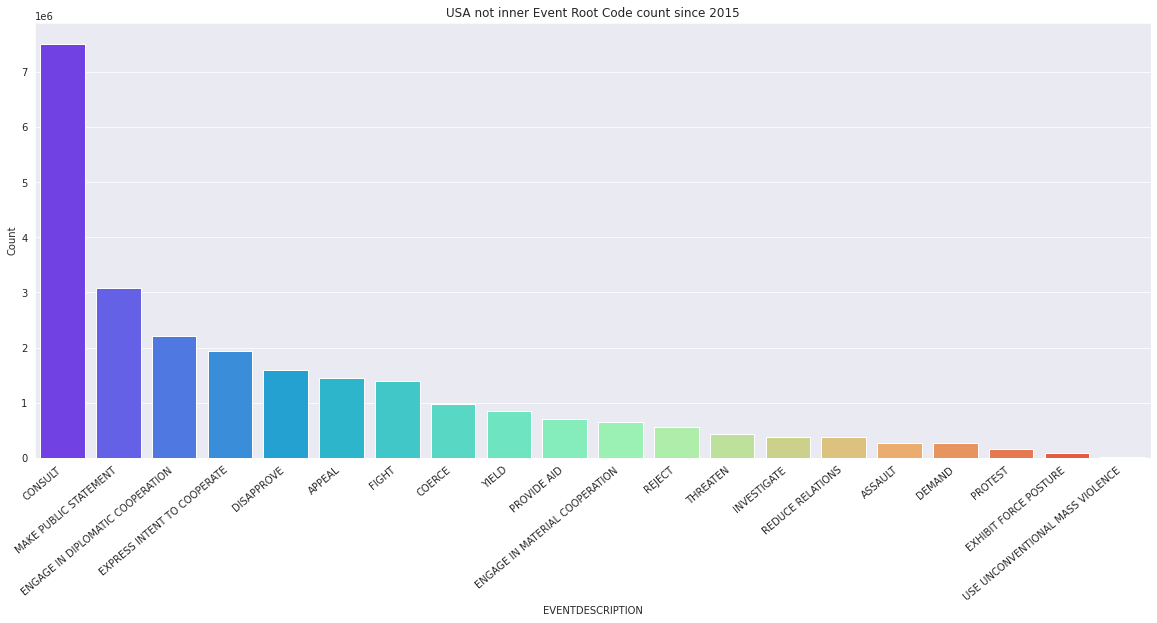
\includegraphics[width=\linewidth]{fig/USA not inner/ERC.png}
        \caption{Liczba zdarzeń zewnętrznych USA dla kodów podstawowych od 2015 - top 20. (źródło: opracowanie własne)}
        \label{fig:USA_not_inner_ERC}
    \end{figure}

    \begin{figure}[!htp]
        \centering
        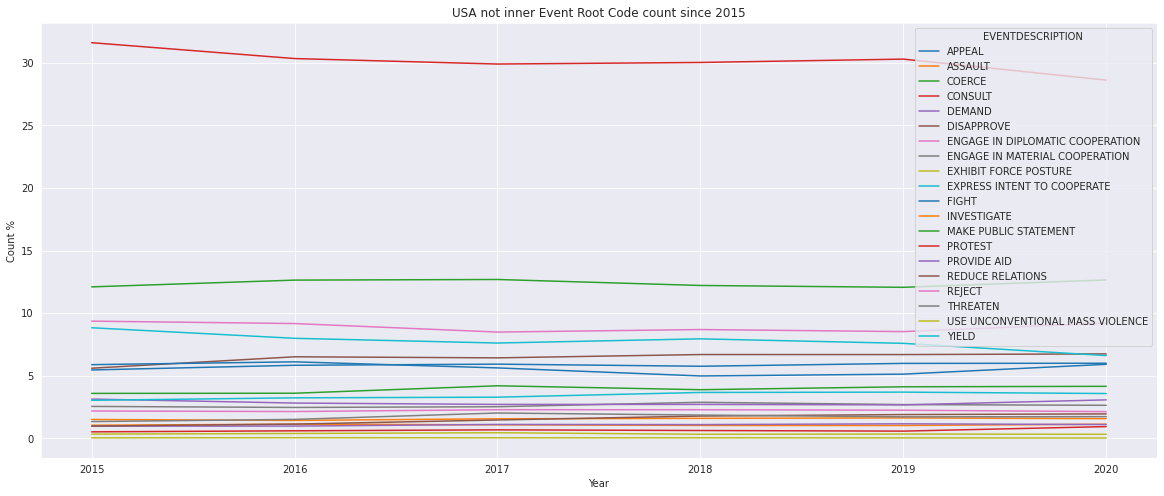
\includegraphics[width=\linewidth]{fig/USA not inner/ERCperc.png}
        \caption{Procentowa liczba zdarzeń zewnętrznych USA dla kodów podstawowych od 2015 - top 10. (źródło: opracowanie własne)}
        \label{fig:USA_not_inner_ERCperc}
    \end{figure}

    Wykres~\ref{fig:GLOBAL_ERC} przedstawia globalną liczbę zdarzeń z poszczególnymi kodami podstawowymi.
    Wykres~\ref{fig:GLOBAL_ERCperc} przedstawiają globalny procentowy udział zdarzeń z poszczególnymi kodami podstawowymi.

    \begin{figure}[!htp]
        \centering
        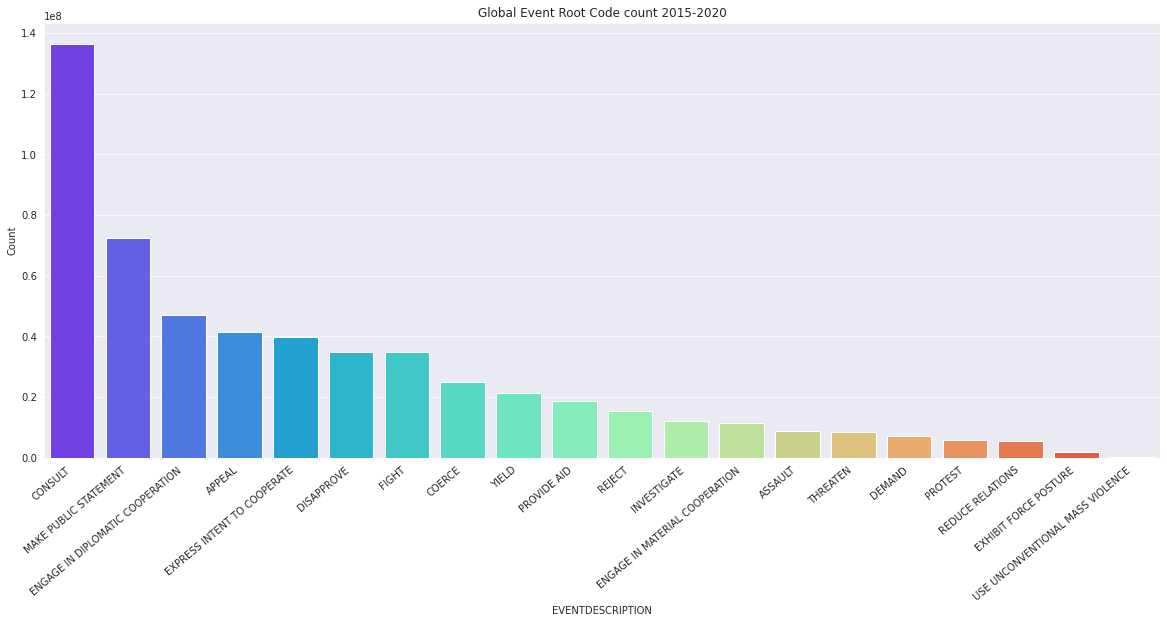
\includegraphics[width=\linewidth]{fig/GLOBAL//ERC.png}
        \caption{Liczba zdarzeń dla kodów podstawowych od 2015 - top 20. (źródło: opracowanie własne)}
        \label{fig:GLOBAL_ERC}
    \end{figure}

    \begin{figure}[!htp]
        \centering
        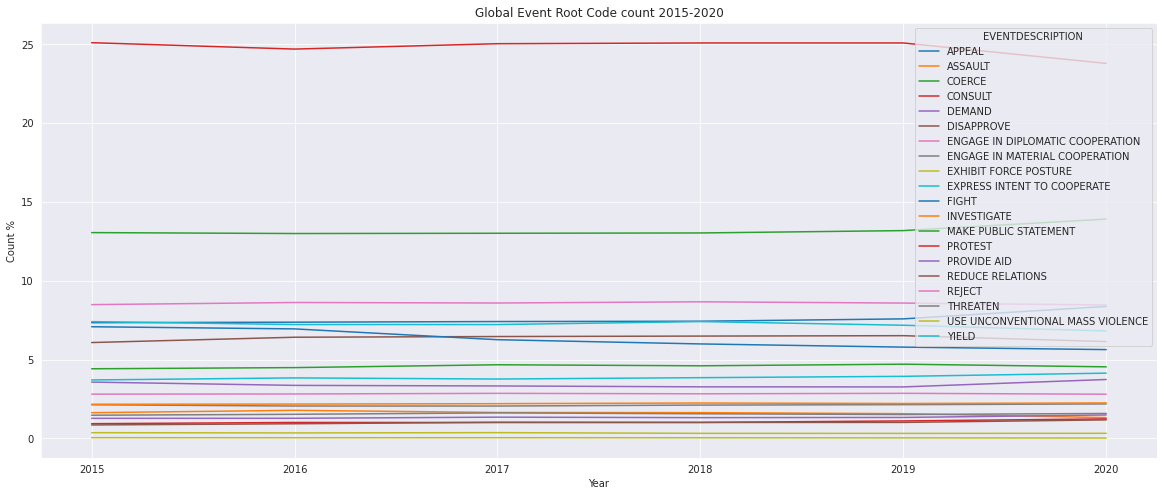
\includegraphics[width=\linewidth]{fig/GLOBAL/ERCperc.png}
        \caption{Procentowa liczba zdarzeń dla kodów podstawowych od 2015 - top 10. (źródło: opracowanie własne)}
        \label{fig:GLOBAL_ERCperc}
    \end{figure}

    Liczba zdarzeń wewnętrznych \textit{Consult} w USA w latach 2015-2020 to około 2,5 miliona.
    Zdarzeń zewnętrznych \textit{Consult} w USA w tym okresie było 3 razy więcej - około 7,5 miliona,
    podczas gdy globalna liczba zdarzeń \textit{Consult} wynosiła około 140 milionów.

    Zarówno dla zdarzeń wewnętrznych USA, zewnętrznych USA jak i globalnych pierwsza trójka wygląda następująco:
    \begin{enumerate}
        \item \textit{Consult},
        \item \textit{Make public statement},
        \item \textit{Engage in diplomatic cooperation}.
    \end{enumerate}

    Takie wyniki wyraźnie świadczą o podobieństwie klasyfikacji podstawowej (Root Codes) zdarzeń.

    \subsection{Czterokody (Quad Class)}

    Wykres~\ref{fig:USA_inner_QC} przedstawia liczbę zdarzeń wewnętrznych w USA z poszczególnymi czterokodami.
    Wykres~\ref{fig:USA_inner_QCperc} przedstawiają procentowy udział zdarzeń wewnętrznych w USA z poszczególnymi czterokodami.

    \begin{figure}[!htp]
        \centering
        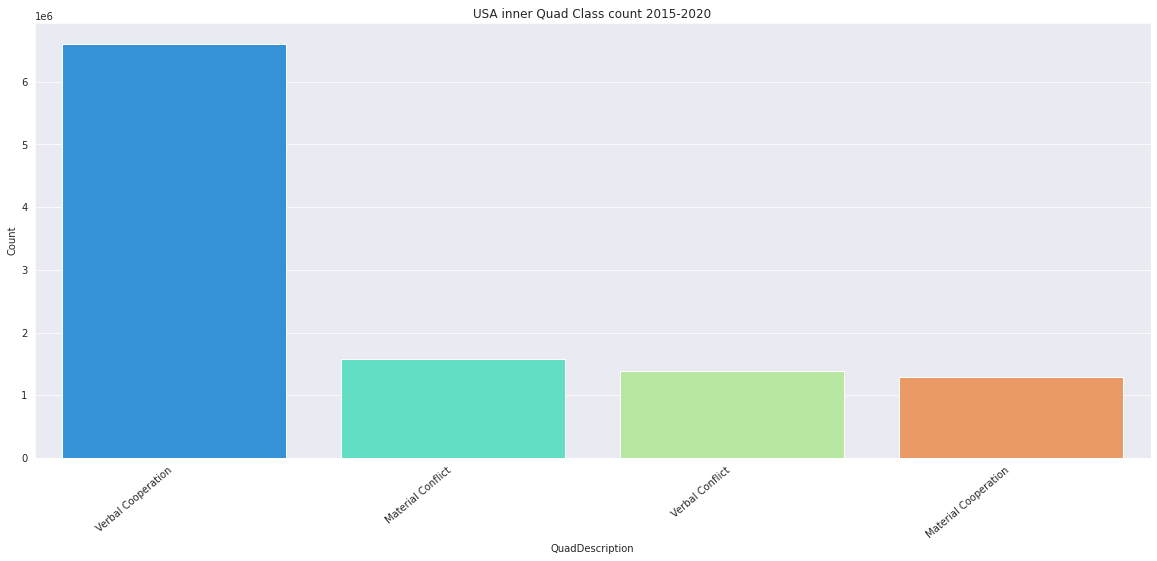
\includegraphics[width=\linewidth]{fig/USA inner/QC.png}
        \caption{Liczba zdarzeń wewnętrznych USA dla czterokodów od 2015. (źródło: opracowanie własne)}
        \label{fig:USA_inner_QC}
    \end{figure}

    \begin{figure}[!htp]
        \centering
        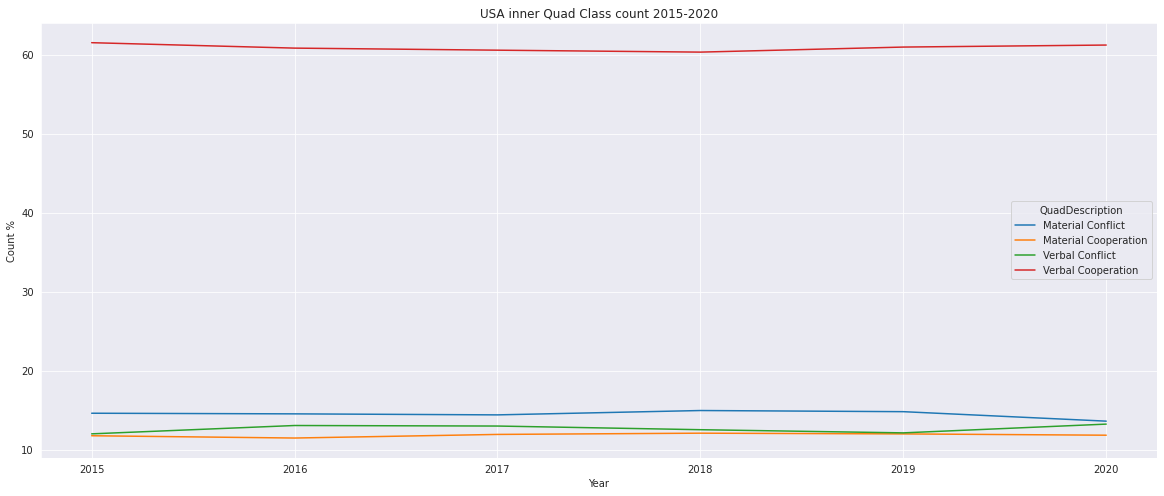
\includegraphics[width=\linewidth]{fig/USA inner/QCperc.png}
        \caption{Procentowa liczba zdarzeń wewnętrznych USA dla czterokodów od 2015 - top 10. (źródło: opracowanie własne)}
        \label{fig:USA_inner_QCperc}
    \end{figure}

    Wykres~\ref{fig:USA_not_inner_QC} przedstawia liczbę zdarzeń pomiędzy USA i innymi krajami z poszczególnymi czterokodami.
    Wykres~\ref{fig:USA_not_inner_QCperc} przedstawiają procentowy udział zdarzeń pomiędzy USA i innymi krajami z poszczególnymi czterokodami.

    \begin{figure}[!htp]
        \centering
        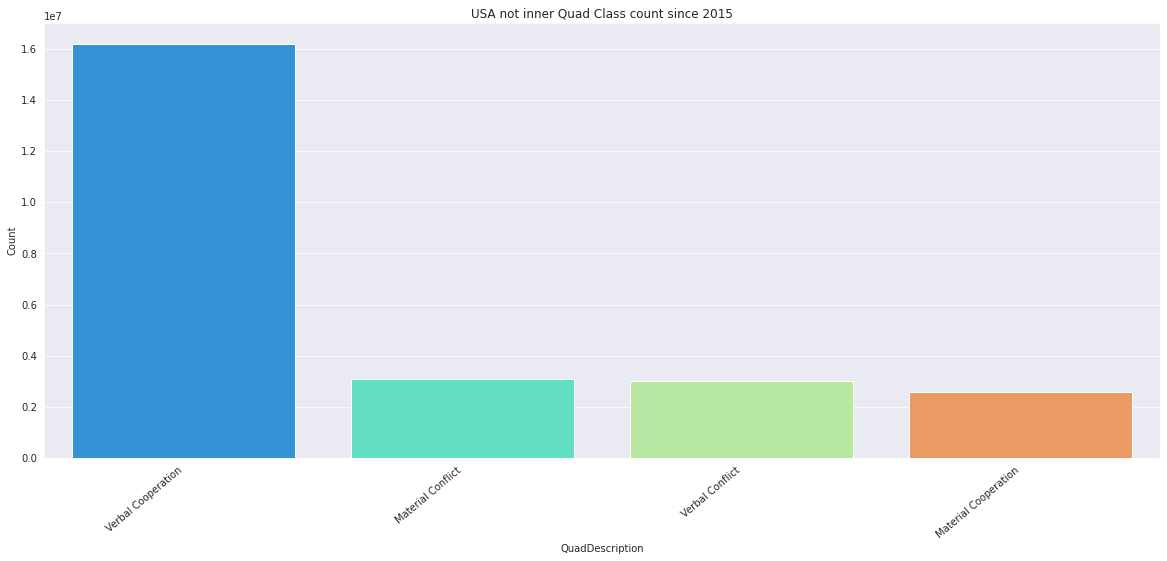
\includegraphics[width=\linewidth]{fig/USA not inner/QC.png}
        \caption{Liczba zdarzeń zewnętrznych USA dla kodów podstawowych od 2015 - top 20. (źródło: opracowanie własne)}
        \label{fig:USA_not_inner_QC}
    \end{figure}

    \begin{figure}[!htp]
        \centering
        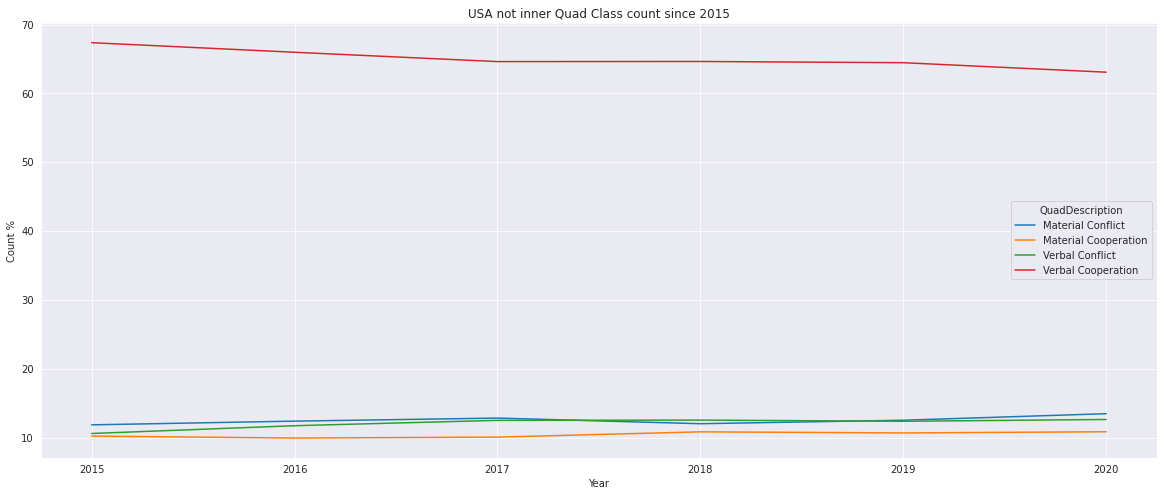
\includegraphics[width=\linewidth]{fig/USA not inner/QCperc.png}
        \caption{Procentowa liczba zdarzeń zewnętrznych USA dla kodów podstawowych od 2015 - top 10. (źródło: opracowanie własne)}
        \label{fig:USA_not_inner_QCperc}
    \end{figure}

    Wykres~\ref{fig:GLOBAL_QC} przedstawia globalną liczbę zdarzeń z poszczególnymi czterokodami.
    Wykres~\ref{fig:GLOBAL_QCperc} przedstawiają globalny procentowy udział zdarzeń z poszczególnymi czterokodami.

    \begin{figure}[!htp]
        \centering
        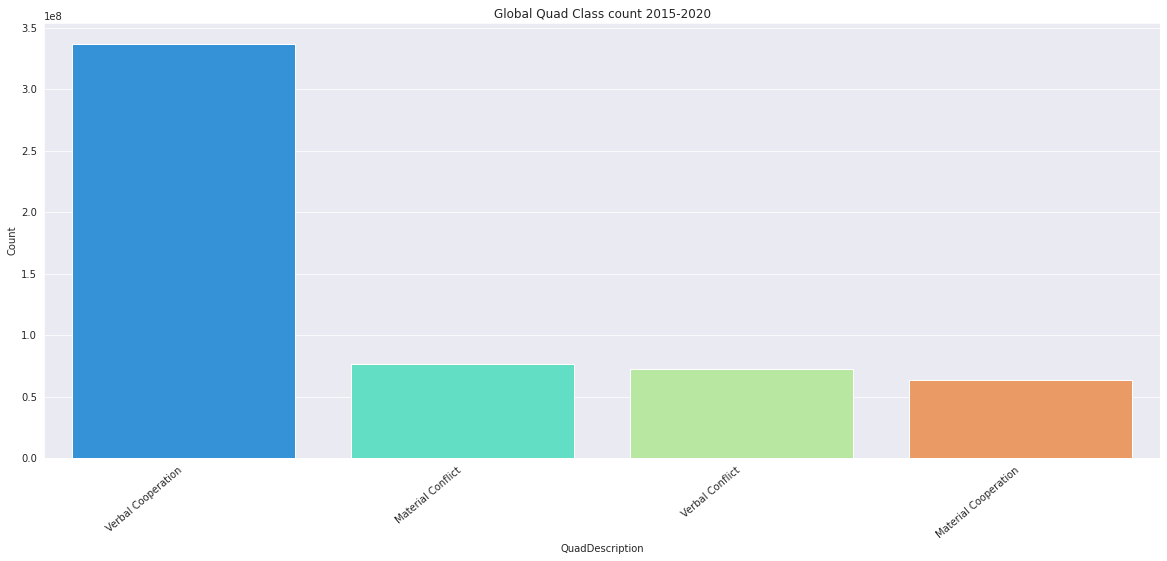
\includegraphics[width=\linewidth]{fig/GLOBAL//QC.png}
        \caption{Liczba zdarzeń dla kodów podstawowych od 2015 - top 20. (źródło: opracowanie własne)}
        \label{fig:GLOBAL_QC}
    \end{figure}

    \begin{figure}[!htp]
        \centering
        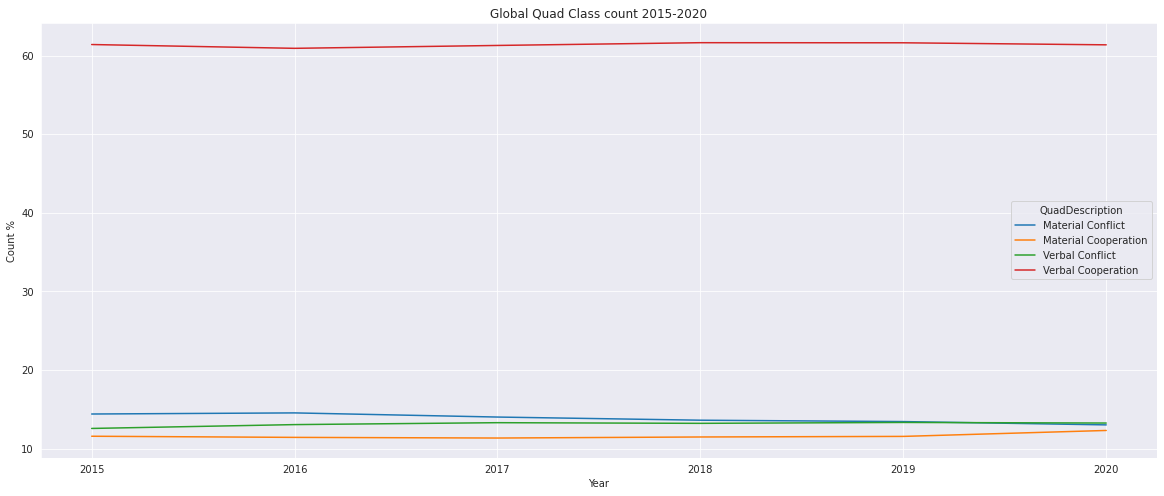
\includegraphics[width=\linewidth]{fig/GLOBAL/QCperc.png}
        \caption{Procentowa liczba zdarzeń dla kodów podstawowych od 2015 - top 10. (źródło: opracowanie własne)}
        \label{fig:GLOBAL_QCperc}
    \end{figure}

    Liczba zdarzeń wewnętrznych \textit{Verbal Cooperation} w USA w latach 2015-2020 to około 6,5 miliona.
    Zdarzeń zewnętrznych \textit{Verbal Cooperation} w USA w tym okresie było 3 razy więcej - około 16 milionów,
    podczas gdy globalna liczba zdarzeń \textit{Verbal Cooperation} wynosiła około 340 milionów.

    Dla wszystkich typów zdarzeń czterokody występują w następującej kolejności:
    \begin{enumerate}
        \item \textit{Verbal Cooperation},
        \item \textit{Material Conflict},
        \item \textit{Verbal Conflict},
        \item \textit{Material Cooperation}.
    \end{enumerate}
    Dla każdego typu zdarzeń przeważającą większość stanowią zdarzenia \textit{Verbal Cooperation}.

    Takie wyniki wyraźnie świadczą o podobieństwie przyporządkowań zdarzeń do czterokodów (Quad Class).


    \chapter{Power-Client analiza wstępna}
    W tym rozdziale przedstawione zostaną wyniki wstępnej analizy mającej na celu wyłonienie miar
    do poszukiwań wzorca Power-Client.


    \section{Event Root Code}

    \subsection{Bez progowania}
    Wykresy~\ref{fig:Power-Client:ERC:POL-USA}, \ref{fig:Power-Client:ERC:POL-RUS} oraz~\ref{fig:Power-Client:ERC:POL-DEU} przedstawiają relacje klient-hegemon.
    \begin{figure}[!htp]
        \centering
        \includegraphics[width=\linewidth]{../Power-Client pre analysis/fig_EventRootCode/POL-USA EventRootCode count 2015-2020 - top 20.png}
        \caption{Procentowa liczba zdarzeń POL-USA wg kodów głównych. (źródło: opracowanie własne)}
        \label{fig:Power-Client:ERC:POL-USA}
    \end{figure}

    \begin{figure}[!htp]
        \centering
        \includegraphics[width=\linewidth]{../Power-Client pre analysis/fig_EventRootCode/POL-RUS EventRootCode count 2015-2020 - top 20.png}
        \caption{Procentowa liczba zdarzeń POL-RUS wg kodów głównych. (źródło: opracowanie własne)}
        \label{fig:Power-Client:ERC:POL-RUS}
    \end{figure}

    \begin{figure}[!htp]
        \centering
        \includegraphics[width=\linewidth]{../Power-Client pre analysis/fig_EventRootCode/POL-DEU EventRootCode count 2015-2020 - top 20.png}
        \caption{Procentowa liczba zdarzeń POL-DEU wg kodów głównych. (źródło: opracowanie własne)}
        \label{fig:Power-Client:ERC:POL-DEU}
    \end{figure}

    Wykresy~\ref{fig:Power-Client:ERC:POL-ESP}, \ref{fig:Power-Client:ERC:POL-CZE} oraz~\ref{fig:Power-Client:ERC:POL-HUN} przedstawiają relacje neutralne.
    \begin{figure}[!htp]
        \centering
        \includegraphics[width=\linewidth]{../Power-Client pre analysis/fig_EventRootCode/POL-ESP EventRootCode count 2015-2020 - top 20.png}
        \caption{Procentowa liczba zdarzeń POL-ESP wg kodów głównych. (źródło: opracowanie własne)}
        \label{fig:Power-Client:ERC:POL-ESP}
    \end{figure}

    \begin{figure}[!htp]
        \centering
        \includegraphics[width=\linewidth]{../Power-Client pre analysis/fig_EventRootCode/POL-CZE EventRootCode count 2015-2020 - top 20.png}
        \caption{Procentowa liczba zdarzeń POL-CZE wg kodów głównych. (źródło: opracowanie własne)}
        \label{fig:Power-Client:ERC:POL-CZE}
    \end{figure}

    \begin{figure}[!htp]
        \centering
        \includegraphics[width=\linewidth]{../Power-Client pre analysis/fig_EventRootCode/POL-HUN EventRootCode count 2015-2020 - top 20.png}
        \caption{Procentowa liczba zdarzeń POL-HUN wg kodów głównych. (źródło: opracowanie własne)}
        \label{fig:Power-Client:ERC:POL-HUN}
    \end{figure}

    Na każdym z 6 wykresów, niezależnie od typu relacji, dominuje liczba zdarzeń \textit{CONSULT}.
    Dla relacji POL-USA oraz POL-RUS na drugim miejscu są zdarzenia \textit{MAKE PUBLIC STATEMENT}.

    \subsection{Próg skala Goldsteina >=3}
    Skala Goldsteina przypisuje każdemu z kodów CAMEO numeryczną wartość od -10 do 10, przedstawia teoretyczny wpływ typu zdarzenia na stabilność kraju.
    Ponieważ skala Goldsteina jest bezpośrednio związana z kodem CAMEO, dlatego filtrowanie wg skali Goldsteina odrzuca cześć kodów.
    Kody CAMEO dla skali Goldsteina >=3 to:
    \begin{itemize}
        \item \textit{ENGAGE IN DIPLOMATIC COOPERATION}
        \item \textit{EXPRESS INTENT TO COOPERATE}
        \item \textit{APPEAL}
        \item \textit{CONSULT}
        \item \textit{YIELD}
        \item \textit{ENGAGE IN MATERIAL COOPERATION}
        \item \textit{PROVIDE AID}
        \item \textit{MAKE PUBLIC CTATEMENT}
    \end{itemize}

    Wykresy~\ref{fig:Power-Client:ERC:Goldstein:POL-USA}, \ref{fig:Power-Client:ERC:Goldstein:POL-RUS} oraz~\ref{fig:Power-Client:ERC:Goldstein:POL-DEU} przedstawiają relacje klient-hegemon.
    \begin{figure}[!htp]
        \centering
        \includegraphics[width=\linewidth]{../Power-Client pre analysis/fig_EventRootCode/POL-USA EventRootCode count 2015-2020 with Goldstein Scale >=3 - top 20.png}
        \caption{Procentowa liczba zdarzeń POL-USA wg kodów głównych. (źródło: opracowanie własne)}
        \label{fig:Power-Client:ERC:Goldstein:POL-USA}
    \end{figure}

    \begin{figure}[!htp]
        \centering
        \includegraphics[width=\linewidth]{../Power-Client pre analysis/fig_EventRootCode/POL-RUS EventRootCode count 2015-2020 with Goldstein Scale >=3 - top 20.png}
        \caption{Procentowa liczba zdarzeń POL-RUS wg kodów głównych. (źródło: opracowanie własne)}
        \label{fig:Power-Client:ERC:Goldstein:POL-RUS}
    \end{figure}

    \begin{figure}[!htp]
        \centering
        \includegraphics[width=\linewidth]{../Power-Client pre analysis/fig_EventRootCode/POL-DEU EventRootCode count 2015-2020 with Goldstein Scale >=3 - top 20.png}
        \caption{Procentowa liczba zdarzeń POL-DEU wg kodów głównych. (źródło: opracowanie własne)}
        \label{fig:Power-Client:ERC:Goldstein:POL-DEU}
    \end{figure}

    Wykresy~\ref{fig:Power-Client:ERC:Goldstein:POL-ESP}, \ref{fig:Power-Client:ERC:Goldstein:POL-CZE} oraz~\ref{fig:Power-Client:ERC:Goldstein:POL-HUN} przedstawiają relacje neutralne.
    \begin{figure}[!htp]
        \centering
        \includegraphics[width=\linewidth]{../Power-Client pre analysis/fig_EventRootCode/POL-ESP EventRootCode count 2015-2020 with Goldstein Scale >=3 - top 20.png}
        \caption{Procentowa liczba zdarzeń POL-ESP wg kodów głównych. (źródło: opracowanie własne)}
        \label{fig:Power-Client:ERC:Goldstein:POL-ESP}
    \end{figure}

    \begin{figure}[!htp]
        \centering
        \includegraphics[width=\linewidth]{../Power-Client pre analysis/fig_EventRootCode/POL-CZE EventRootCode count 2015-2020 with Goldstein Scale >=3 - top 20.png}
        \caption{Procentowa liczba zdarzeń POL-CZE wg kodów głównych. (źródło: opracowanie własne)}
        \label{fig:Power-Client:ERC:Goldstein:POL-CZE}
    \end{figure}

    \begin{figure}[!htp]
        \centering
        \includegraphics[width=\linewidth]{../Power-Client pre analysis/fig_EventRootCode/POL-HUN EventRootCode count 2015-2020 with Goldstein Scale >=3 - top 20.png}
        \caption{Procentowa liczba zdarzeń POL-HUN wg kodów głównych. (źródło: opracowanie własne)}
        \label{fig:Power-Client:ERC:Goldstein:POL-HUN}
    \end{figure}

    Na każdym z 6 wykresów, niezależnie od typu relacji, dominuje liczba zdarzeń \textit{ENGAGE IN DIPLOMATIC COOPERATION}.
    Dla wszystkich relacji, z wyjątkiem POL-RUS, na drugim miejscu są zdarzenia \textit{EXPRESS INTENT TO COOPERATE}.

    \subsection{Próg ilość wzmianek >=5}
    Liczba wzmianek to całkowita liczba wystąpień informacji o danym zdarzeniu pośród dokumentów źródłowych.
    Pozwala określić ważność danego zdarzenia.
    Im więcej dyskusji o danym zdarzeniu, tym bardziej prawdopodobne, że jest ono istotne.

    Wykresy~\ref{fig:Power-Client:ERC:Mentions:POL-USA}, \ref{fig:Power-Client:ERC:Mentions:POL-RUS} oraz~\ref{fig:Power-Client:ERC:Mentions:POL-DEU} przedstawiają relacje klient-hegemon.
    \begin{figure}[!htp]
        \centering
        \includegraphics[width=\linewidth]{../Power-Client pre analysis/fig_EventRootCode/POL-USA EventRootCode count 2015-2020 with mentions >=5 - top 20.png}
        \caption{Procentowa liczba zdarzeń POL-USA wg kodów głównych. (źródło: opracowanie własne)}
        \label{fig:Power-Client:ERC:Mentions:POL-USA}
    \end{figure}

    \begin{figure}[!htp]
        \centering
        \includegraphics[width=\linewidth]{../Power-Client pre analysis/fig_EventRootCode/POL-RUS EventRootCode count 2015-2020 with mentions >=5 - top 20.png}
        \caption{Procentowa liczba zdarzeń POL-RUS wg kodów głównych. (źródło: opracowanie własne)}
        \label{fig:Power-Client:ERC:Mentions:POL-RUS}
    \end{figure}

    \begin{figure}[!htp]
        \centering
        \includegraphics[width=\linewidth]{../Power-Client pre analysis/fig_EventRootCode/POL-DEU EventRootCode count 2015-2020 with mentions >=5 - top 20.png}
        \caption{Procentowa liczba zdarzeń POL-DEU wg kodów głównych. (źródło: opracowanie własne)}
        \label{fig:Power-Client:ERC:Mentions:POL-DEU}
    \end{figure}

    Wykresy~\ref{fig:Power-Client:ERC:Mentions:POL-ESP}, \ref{fig:Power-Client:ERC:Mentions:POL-CZE} oraz~\ref{fig:Power-Client:ERC:Mentions:POL-HUN} przedstawiają relacje neutralne.
    \begin{figure}[!htp]
        \centering
        \includegraphics[width=\linewidth]{../Power-Client pre analysis/fig_EventRootCode/POL-ESP EventRootCode count 2015-2020 with mentions >=5 - top 20.png}
        \caption{Procentowa liczba zdarzeń POL-ESP wg kodów głównych. (źródło: opracowanie własne)}
        \label{fig:Power-Client:ERC:Mentions:POL-ESP}
    \end{figure}

    \begin{figure}[!htp]
        \centering
        \includegraphics[width=\linewidth]{../Power-Client pre analysis/fig_EventRootCode/POL-CZE EventRootCode count 2015-2020 with mentions >=5 - top 20.png}
        \caption{Procentowa liczba zdarzeń POL-CZE wg kodów głównych. (źródło: opracowanie własne)}
        \label{fig:Power-Client:ERC:Mentions:POL-CZE}
    \end{figure}

    \begin{figure}[!htp]
        \centering
        \includegraphics[width=\linewidth]{../Power-Client pre analysis/fig_EventRootCode/POL-HUN EventRootCode count 2015-2020 with mentions >=5 - top 20.png}
        \caption{Procentowa liczba zdarzeń POL-HUN wg kodów głównych. (źródło: opracowanie własne)}
        \label{fig:Power-Client:ERC:Mentions:POL-HUN}
    \end{figure}

    Na każdym z 6 wykresów, niezależnie od typu relacji, dominuje liczba zdarzeń \textit{CONSULT}.
    Dla wszystkich relacji, z wyjątkiem POL-RUS, na drugim miejscu są zdarzenia \textit{ENGAGE IN DIPLOMATIC COOPERATION}.

    \paragraph{Wnioski}
    Kody główne zdarzeń wydają się być zbyt ogólne do wyróżniania relacji typu mocarstwo-klient.


    \section{Event Base Code}\label{sec:event-base-code}

    \subsection{Bez progowania}
    Wykresy~\ref{fig:Power-Client:EBC:POL-USA}, \ref{fig:Power-Client:EBC:POL-RUS} oraz~\ref{fig:Power-Client:EBC:POL-DEU} przedstawiają relacje klient-hegemon.
    \begin{figure}[!htp]
        \centering
        \includegraphics[width=\linewidth]{../Power-Client pre analysis/fig_EventBaseCode/POL-USA EventBaseCode count 2015-2020 - top 20.png}
        \caption{Procentowa liczba zdarzeń POL-USA wg kodów głównych. (źródło: opracowanie własne)}
        \label{fig:Power-Client:EBC:POL-USA}
    \end{figure}

    \begin{figure}[!htp]
        \centering
        \includegraphics[width=\linewidth]{../Power-Client pre analysis/fig_EventBaseCode/POL-RUS EventBaseCode count 2015-2020 - top 20.png}
        \caption{Procentowa liczba zdarzeń POL-RUS wg kodów głównych. (źródło: opracowanie własne)}
        \label{fig:Power-Client:EBC:POL-RUS}
    \end{figure}

    \begin{figure}[!htp]
        \centering
        \includegraphics[width=\linewidth]{../Power-Client pre analysis/fig_EventBaseCode/POL-DEU EventBaseCode count 2015-2020 - top 20.png}
        \caption{Procentowa liczba zdarzeń POL-DEU wg kodów głównych. (źródło: opracowanie własne)}
        \label{fig:Power-Client:EBC:POL-DEU}
    \end{figure}

    Wykresy~\ref{fig:Power-Client:EBC:POL-ESP}, \ref{fig:Power-Client:EBC:POL-CZE} oraz~\ref{fig:Power-Client:EBC:POL-HUN} przedstawiają relacje neutralne.
    \begin{figure}[!htp]
        \centering
        \includegraphics[width=\linewidth]{../Power-Client pre analysis/fig_EventBaseCode/POL-ESP EventBaseCode count 2015-2020 - top 20.png}
        \caption{Procentowa liczba zdarzeń POL-ESP wg kodów głównych. (źródło: opracowanie własne)}
        \label{fig:Power-Client:EBC:POL-ESP}
    \end{figure}

    \begin{figure}[!htp]
        \centering
        \includegraphics[width=\linewidth]{../Power-Client pre analysis/fig_EventBaseCode/POL-CZE EventBaseCode count 2015-2020 - top 20.png}
        \caption{Procentowa liczba zdarzeń POL-CZE wg kodów głównych. (źródło: opracowanie własne)}
        \label{fig:Power-Client:EBC:POL-CZE}
    \end{figure}

    \begin{figure}[!htp]
        \centering
        \includegraphics[width=\linewidth]{../Power-Client pre analysis/fig_EventBaseCode/POL-HUN EventBaseCode count 2015-2020 - top 20.png}
        \caption{Procentowa liczba zdarzeń POL-HUN wg kodów głównych. (źródło: opracowanie własne)}
        \label{fig:Power-Client:EBC:POL-HUN}
    \end{figure}

    Dla relacji POL-USA oraz POL-DEU na pierwszym miejscu występują zdarzenia \textit{Make a visit}, a następnie
    \textit{Host a visit} oraz \textit{Consult- not specific below}.
    Dla relacji POL-CZE oraz POL-HUN na pierwszym miejscu występują zdarzenia \textit{Consult - not specified below}.

    \subsubsection{Wybrane wykresy podsumowujące}
    Ta sekcja przedstawia ręcznie wybrane wykresy podsumowujące zawierające przynajmniej 8 krajów.
    Kryterium wyboru była zauważalna separacja relacji klient-hegemon oraz neutralnych.

    \begin{figure}[!htp]
        \centering
        \includegraphics[width=\linewidth]{../Power-Client pre analysis/fig_EventBaseCode_event_sum_up/Engage in negotiation events 2015-2020 .png}
        \caption{Procentowa liczba zdarzeń Engage in negotiation dla poszczególnych krajów. (źródło: opracowanie własne)}
        \label{fig:Power-Client:ERC:SumUp:Engage in negotiation}
    \end{figure}
    Na wykresie~\ref{fig:Power-Client:ERC:SumUp:Engage in negotiation} Niemcy, USA oraz Rosja są w jednej grupie,
    charakteryzującej się najmniejszą procentową ilością zdarzeń \textit{Engage in negotiation}.
    Na podstawie tego wykresu zbiorczego~\ref{fig:Power-Client:ERC:SumUp:Engage in negotiation}
    jest bardzo dobry kandydatem na jedną z miar przy klastrowaniu.

    \begin{figure}[!htp]
        \centering
        \includegraphics[width=\linewidth]{../Power-Client pre analysis/fig_EventBaseCode_event_sum_up/Make statement- not specified below events 2015-2020 .png}
        \caption{Procentowa liczba zdarzeń Make statement- not specified below dla poszczególnych krajów. (źródło: opracowanie własne)}
        \label{fig:Power-Client:ERC:SumUp:Make statement - not specified below}
    \end{figure}
    Na wykresie~\ref{fig:Power-Client:ERC:SumUp:Make statement - not specified below} USA oraz Rosja są w jednej grupie,
    charakteryzującej się największą procentową ilością zdarzeń \textit{Make statement - not specified below}.
    Rosję i USA dzieli od pozostałych krajów wyraźna różnica.
    Niemcy oddzielone są od Rosji i USA przez Białoruś i Ukrainę.

    Pozostałe typy zdarzeń znacznie gorzej rozdzielają relacje klient-hegemon oraz neutralne wśród analizowanych krajów.

    \subsection{Próg skala Goldsteina >=3}
    Skala Goldsteina przypisuje każdemu z kodów CAMEO numeryczną wartość od -10 do 10, przedstawia teoretyczny wpływ typu zdarzenia na stabilność kraju.
    Ponieważ skala Goldsteina jest bezpośrednio związana z kodem CAMEO, dlatego filtrowanie wg skali Goldsteina odrzuca część kodów.

    Wykresy~\ref{fig:Power-Client:EBC:Goldstein:POL-USA},~\ref{fig:Power-Client:EBC:Goldstein:POL-RUS} oraz~\ref{fig:Power-Client:EBC:Goldstein:POL-DEU} przedstawiają relacje klient-hegemon.
    \begin{figure}[!htp]
        \centering
        \includegraphics[width=\linewidth]{../Power-Client pre analysis/fig_EventBaseCode/POL-USA EventBaseCode count 2015-2020 with Goldstein Scale >=3 - top 20.png}
        \caption{Procentowa liczba zdarzeń POL-USA wg kodów głównych. (źródło: opracowanie własne)}
        \label{fig:Power-Client:EBC:Goldstein:POL-USA}
    \end{figure}

    \begin{figure}[!htp]
        \centering
        \includegraphics[width=\linewidth]{../Power-Client pre analysis/fig_EventBaseCode/POL-RUS EventBaseCode count 2015-2020 with Goldstein Scale >=3 - top 20.png}
        \caption{Procentowa liczba zdarzeń POL-RUS wg kodów głównych. (źródło: opracowanie własne)}
        \label{fig:Power-Client:EBC:Goldstein:POL-RUS}
    \end{figure}

    \begin{figure}[!htp]
        \centering
        \includegraphics[width=\linewidth]{../Power-Client pre analysis/fig_EventBaseCode/POL-DEU EventBaseCode count 2015-2020 with Goldstein Scale >=3 - top 20.png}
        \caption{Procentowa liczba zdarzeń POL-DEU wg kodów głównych. (źródło: opracowanie własne)}
        \label{fig:Power-Client:EBC:Goldstein:POL-DEU}
    \end{figure}

    Wykresy~\ref{fig:Power-Client:EBC:Goldstein:POL-ESP},~\ref{fig:Power-Client:EBC:Goldstein:POL-CZE} oraz~\ref{fig:Power-Client:EBC:Goldstein:POL-HUN} przedstawiają relacje neutralne.
    \begin{figure}[!htp]
        \centering
        \includegraphics[width=\linewidth]{../Power-Client pre analysis/fig_EventBaseCode/POL-ESP EventBaseCode count 2015-2020 with Goldstein Scale >=3 - top 20.png}
        \caption{Procentowa liczba zdarzeń POL-ESP wg kodów głównych. (źródło: opracowanie własne)}
        \label{fig:Power-Client:EBC:Goldstein:POL-ESP}
    \end{figure}

    \begin{figure}[!htp]
        \centering
        \includegraphics[width=\linewidth]{../Power-Client pre analysis/fig_EventBaseCode/POL-CZE EventBaseCode count 2015-2020 with Goldstein Scale >=3 - top 20.png}
        \caption{Procentowa liczba zdarzeń POL-CZE wg kodów głównych. (źródło: opracowanie własne)}
        \label{fig:Power-Client:EBC:Goldstein:POL-CZE}
    \end{figure}

    \begin{figure}[!htp]
        \centering
        \includegraphics[width=\linewidth]{../Power-Client pre analysis/fig_EventBaseCode/POL-HUN EventBaseCode count 2015-2020 with Goldstein Scale >=3 - top 20.png}
        \caption{Procentowa liczba zdarzeń POL-HUN wg kodów głównych. (źródło: opracowanie własne)}
        \label{fig:Power-Client:EBC:Goldstein:POL-HUN}
    \end{figure}

    \subsubsection{Wybrane wykresy podsumowujące}
    Ta sekcja przedstawia ręcznie wybrane wykresy podsumowujące zawierające przynajmniej 8 krajów.
    Kryterium wyboru była zauważalna separacja relacji klient-hegemon oraz neutralnych.

    \begin{figure}[!htp]
        \centering
        \includegraphics[width=\linewidth]{../Power-Client pre analysis/fig_EventBaseCodeGoldstein Scale >=3 _event_sum_up/Express intent to cooperate- not specified below events 2015-2020 Goldstein Scale >=3 .png}
        \caption{Procentowa liczba zdarzeń Express intent to cooperate- not specified below dla poszczególnych krajów. (źródło: opracowanie własne)}
        \label{fig:Power-Client:ERC:Goldstein:SumUp:Express intent to cooperate- not specified below}
    \end{figure}
    Na wykresie~\ref{fig:Power-Client:ERC:Goldstein:SumUp:Express intent to cooperate- not specified below} Niemcy, USA oraz Rosja są w jednej grupie,
    charakteryzującej się niską procentową ilością zdarzeń \textit{Express intent to cooperate- not specified belo}.
    Do tej samej grupy należą też Hiszpania i Włochy.

    \begin{figure}[!htp]
        \centering
        \includegraphics[width=\linewidth]{../Power-Client pre analysis/fig_EventBaseCodeGoldstein Scale >=3 _event_sum_up/Return release- not specified below events 2015-2020 Goldstein Scale >=3 .png}
        \caption{Procentowa liczba zdarzeń Return release- not specified below dla poszczególnych krajów. (źródło: opracowanie własne)}
        \label{fig:Power-Client:ERC:Goldstein:SumUp:Return release- not specified below}
    \end{figure}
    Na wykresie~\ref{fig:Power-Client:ERC:Goldstein:SumUp:Return release- not specified below} USA oraz Rosja są w jednej grupie,
    charakteryzującej się największą procentową ilością zdarzeń \textit{Return release- not specified below}.
    Do tej samej grupy należy też Ukraina która oddziela od Niemycy od Rosji i USA.
    Pomiędzy Rosją, a pozostałymi krajami jest wyraźna różnica.
    Grupa krajów z największą procentową ilością zdarzeń jest wyraźnie oddzielona od reszty krajów.

    Pozostałe typy zdarzeń znacznie gorzej rozdzielają relacje klient-hegemon oraz neutralne wśród analizowanych krajów.

    \subsection{Próg ilość wzmianek >=5}
    Liczba wzmianek to całkowita liczba wystąpień informacji o danym zdarzeniu pośród dokumentów źródłowych.
    Pozwala określić ważność danego zdarzenia.
    Im więcej dyskusji o danym zdarzeniu, tym bardziej prawdopodobne, że jest ono istotne.

    Wykresy~\ref{fig:Power-Client:EBC:Mentions:POL-USA}, \ref{fig:Power-Client:EBC:Mentions:POL-RUS} oraz~\ref{fig:Power-Client:EBC:Mentions:POL-DEU} przedstawiają relacje klient-hegemon.
    \begin{figure}[!htp]
        \centering
        \includegraphics[width=\linewidth]{../Power-Client pre analysis/fig_EventBaseCode/POL-USA EventBaseCode count 2015-2020 with mentions >=5 - top 20.png}
        \caption{Procentowa liczba zdarzeń POL-USA wg kodów głównych. (źródło: opracowanie własne)}
        \label{fig:Power-Client:EBC:Mentions:POL-USA}
    \end{figure}

    \begin{figure}[!htp]
        \centering
        \includegraphics[width=\linewidth]{../Power-Client pre analysis/fig_EventBaseCode/POL-RUS EventBaseCode count 2015-2020 with mentions >=5 - top 20.png}
        \caption{Procentowa liczba zdarzeń POL-RUS wg kodów głównych. (źródło: opracowanie własne)}
        \label{fig:Power-Client:EBC:Mentions:POL-RUS}
    \end{figure}

    \begin{figure}[!htp]
        \centering
        \includegraphics[width=\linewidth]{../Power-Client pre analysis/fig_EventBaseCode/POL-DEU EventBaseCode count 2015-2020 with mentions >=5 - top 20.png}
        \caption{Procentowa liczba zdarzeń POL-DEU wg kodów głównych. (źródło: opracowanie własne)}
        \label{fig:Power-Client:EBC:Mentions:POL-DEU}
    \end{figure}

    Wykresy~\ref{fig:Power-Client:EBC:Mentions:POL-ESP}, \ref{fig:Power-Client:EBC:Mentions:POL-CZE} oraz~\ref{fig:Power-Client:EBC:Mentions:POL-HUN} przedstawiają relacje neutralne.
    \begin{figure}[!htp]
        \centering
        \includegraphics[width=\linewidth]{../Power-Client pre analysis/fig_EventBaseCode/POL-ESP EventBaseCode count 2015-2020 with mentions >=5 - top 20.png}
        \caption{Procentowa liczba zdarzeń POL-ESP wg kodów głównych. (źródło: opracowanie własne)}
        \label{fig:Power-Client:EBC:Mentions:POL-ESP}
    \end{figure}

    \begin{figure}[!htp]
        \centering
        \includegraphics[width=\linewidth]{../Power-Client pre analysis/fig_EventBaseCode/POL-CZE EventBaseCode count 2015-2020 with mentions >=5 - top 20.png}
        \caption{Procentowa liczba zdarzeń POL-CZE wg kodów głównych. (źródło: opracowanie własne)}
        \label{fig:Power-Client:EBC:Mentions:POL-CZE}
    \end{figure}

    \begin{figure}[!htp]
        \centering
        \includegraphics[width=\linewidth]{../Power-Client pre analysis/fig_EventBaseCode/POL-HUN EventBaseCode count 2015-2020 with mentions >=5 - top 20.png}
        \caption{Procentowa liczba zdarzeń POL-HUN wg kodów głównych. (źródło: opracowanie własne)}
        \label{fig:Power-Client:EBC:Mentions:POL-HUN}
    \end{figure}

    Dla relacji POL-CZE oraz POL-HUN na pierwszym miejscu, z wyraźną przewagą, występują zdarzenia \textit{Consult - not specified below}.

    \subsubsection{Wybrane wykresy podsumowujące}
    Ta sekcja przedstawia ręcznie wybrane wykresy podsumowujące zawierające przynajmniej 8 krajów.
    Kryterium wyboru była zauważalna separacja relacji klient-hegemon oraz neutralnych.

    \begin{figure}[!htp]
        \centering
        \includegraphics[width=\linewidth]{../Power-Client pre analysis/fig_EventBaseCodewith mentions >=5_event_sum_up/Consult- not specified below events 2015-2020 with mentions >=5.png}
        \caption{Procentowa liczba zdarzeń Consult- not specified below dla poszczególnych krajów. (źródło: opracowanie własne)}
        \label{fig:Power-Client:ERC:Mentions:SumUp:Consult- not specified below}
    \end{figure}
    Na wykresie~\ref{fig:Power-Client:ERC:Mentions:SumUp:Consult- not specified below} Niemcy, USA oraz Rosja są w grupie,
    charakteryzującej się niską procentową ilością zdarzeń \textit{Consult- not specified below}.
    Grupa to nie jest wyraźnie oddzielona od pozostałych.
    Należą do niej też Włochy i Hiszpania - tak jak w przypadku zdarzeń~\textit{Express intent to cooperate- not specified below}
    na wykresie~\ref{fig:Power-Client:ERC:Goldstein:SumUp:Express intent to cooperate- not specified below}.

    \begin{figure}[!htp]
        \centering
        \includegraphics[width=\linewidth]{../Power-Client pre analysis/fig_EventBaseCodewith mentions >=5_event_sum_up/Engage in negotiation events 2015-2020 with mentions >=5.png}
        \caption{Procentowa liczba zdarzeń Engage in negotiation dla poszczególnych krajów. (źródło: opracowanie własne)}
        \label{fig:Power-Client:ERC:Mentions:SumUp:Engage in negotiation}
    \end{figure}
    Na wykresie~\ref{fig:Power-Client:ERC:Mentions:SumUp:Engage in negotiation} Niemcy, USA oraz Rosja są w grupie,
    charakteryzującej się niską procentową ilością zdarzeń \textit{Engage in negotiation}.
    Ponownie do tej samej grupy należą również Włochy i Hiszpania.

    \begin{figure}[!htp]
        \centering
        \includegraphics[width=\linewidth]{../Power-Client pre analysis/fig_EventBaseCodewith mentions >=5_event_sum_up/Use conventional military force- not specified below events 2015-2020 with mentions >=5.png}
        \caption{Procentowa liczba zdarzeń Use conventional military force- not specified below dla poszczególnych krajów. (źródło: opracowanie własne)}
        \label{fig:Power-Client:ERC:Goldstein:SumUp:Use conventional military force- not specified below}
    \end{figure}
    Na wykresie~\ref{fig:Power-Client:ERC:Goldstein:SumUp:Use conventional military force- not specified below} Niemcy, USA oraz Rosja są w grupie,
    charakteryzującej się największą procentową ilością zdarzeń \textit{Use conventional military force- not specified below}.
    Dominacja Niemiec w tym zestawieniu jest najprawdopodobniej spowodowana kontrowersyjnymi kwestiami historycznymi
    które często pojawiają się w relacji Polski i Niemiec.
    Drugie miejsce Hiszpani - która rozdziela Niemcy i USA - wymaga dalszej analizy.

    Pozostałe typy zdarzeń znacznie gorzej rozdzielają relacje klient-hegemon oraz neutralne wśród analizowanych krajów.

    \subsection{Próg ilość wzmianek >=10}
    Liczba wzmianek to całkowita liczba wystąpień informacji o danym zdarzeniu pośród dokumentów źródłowych.
    Pozwala określić ważność danego zdarzenia.
    Im więcej dyskusji o danym zdarzeniu, tym bardziej prawdopodobne, że jest ono istotne.

    Wykresy~\ref{fig:Power-Client:EBC:Mentions10:POL-USA}, \ref{fig:Power-Client:EBC:Mentions10:POL-RUS} oraz~\ref{fig:Power-Client:EBC:Mentions10:POL-DEU} przedstawiają relacje klient-hegemon.
    \begin{figure}[!htp]
        \centering
        \includegraphics[width=\linewidth]{../Power-Client pre analysis/fig_EventBaseCode/POL-USA EventBaseCode count 2015-2020 with mentions >=10 - top 20.png}
        \caption{Procentowa liczba zdarzeń POL-USA wg kodów głównych. (źródło: opracowanie własne)}
        \label{fig:Power-Client:EBC:Mentions10:POL-USA}
    \end{figure}

    \begin{figure}[!htp]
        \centering
        \includegraphics[width=\linewidth]{../Power-Client pre analysis/fig_EventBaseCode/POL-RUS EventBaseCode count 2015-2020 with mentions >=10 - top 20.png}
        \caption{Procentowa liczba zdarzeń POL-RUS wg kodów głównych. (źródło: opracowanie własne)}
        \label{fig:Power-Client:EBC:Mentions10:POL-RUS}
    \end{figure}

    \begin{figure}[!htp]
        \centering
        \includegraphics[width=\linewidth]{../Power-Client pre analysis/fig_EventBaseCode/POL-DEU EventBaseCode count 2015-2020 with mentions >=10 - top 20.png}
        \caption{Procentowa liczba zdarzeń POL-DEU wg kodów głównych. (źródło: opracowanie własne)}
        \label{fig:Power-Client:EBC:Mentions10:POL-DEU}
    \end{figure}

    Wykresy~\ref{fig:Power-Client:EBC:Mentions10:POL-ESP}, \ref{fig:Power-Client:EBC:Mentions10:POL-CZE} oraz~\ref{fig:Power-Client:EBC:Mentions10:POL-HUN} przedstawiają relacje neutralne.
    \begin{figure}[!htp]
        \centering
        \includegraphics[width=\linewidth]{../Power-Client pre analysis/fig_EventBaseCode/POL-ESP EventBaseCode count 2015-2020 with mentions >=10 - top 20.png}
        \caption{Procentowa liczba zdarzeń POL-ESP wg kodów głównych. (źródło: opracowanie własne)}
        \label{fig:Power-Client:EBC:Mentions10:POL-ESP}
    \end{figure}

    \begin{figure}[!htp]
        \centering
        \includegraphics[width=\linewidth]{../Power-Client pre analysis/fig_EventBaseCode/POL-CZE EventBaseCode count 2015-2020 with mentions >=10 - top 20.png}
        \caption{Procentowa liczba zdarzeń POL-CZE wg kodów głównych. (źródło: opracowanie własne)}
        \label{fig:Power-Client:EBC:Mentions10:POL-CZE}
    \end{figure}

    \begin{figure}[!htp]
        \centering
        \includegraphics[width=\linewidth]{../Power-Client pre analysis/fig_EventBaseCode/POL-HUN EventBaseCode count 2015-2020 with mentions >=10 - top 20.png}
        \caption{Procentowa liczba zdarzeń POL-HUN wg kodów głównych. (źródło: opracowanie własne)}
        \label{fig:Power-Client:EBC:Mentions10:POL-HUN}
    \end{figure}

    Dla relacji POL-CZE oraz POL-HUN na pierwszym miejscu występują zdarzenia \textit{Consult - not specified below}.

    \subsubsection{Wybrane wykresy podsumowujące}
    Ta sekcja przedstawia ręcznie wybrane wykresy podsumowujące zawierające przynajmniej 8 krajów.
    Kryterium wyboru była zauważalna separacja relacji klient-hegemon oraz neutralnych.

    \begin{figure}[!htp]
        \centering
        \includegraphics[width=\linewidth]{../Power-Client pre analysis/fig_EventBaseCodewith mentions >=10_event_sum_up/Praise or endorse events 2015-2020 with mentions >=10.png}
        \caption{Procentowa liczba zdarzeń Praise or endorse dla poszczególnych krajów. (źródło: opracowanie własne)}
        \label{fig:Power-Client:ERC:Mentions10:SumUp:Praise or endorse}
    \end{figure}
    Na wykresie~\ref{fig:Power-Client:ERC:Mentions10:SumUp:Praise or endorse} Niemcy, USA oraz Rosja są w grupie,
    charakteryzującej się niską procentową ilością zdarzeń \textit{Praise or endorse}.

    \textit{Praise or endorse} jest jedynym typem zdarzeń który dobrze rozdziela relacje klient-hegemon od neutralnych
    przy progowaniu liczby wzmianek >=10.

    \subsection{Próg średniego tonu >=10 lub <=-10}
    Średni ton to średnia dla wszystkich dokumentów zawierających wzmiankę o danym wydarzeniu.
    Ocena od -100 (ekstremalnie negatywna) do 100 (ekstremalnie pozytywna).
    Ekstremalny ton sugeruje bardziej poważne zdarzenie.

    Wykresy~\ref{fig:Power-Client:EBC:AvgToone10:POL-USA}, \ref{fig:Power-Client:EBC:AvgToone10:POL-RUS} oraz~\ref{fig:Power-Client:EBC:AvgToone10:POL-DEU} przedstawiają relacje klient-hegemon.
    \begin{figure}[!htp]
        \centering
        \includegraphics[width=\linewidth]{../Power-Client pre analysis/fig_EventBaseCode/POL-USA EventBaseCode count 2015-2020 with AvgTone >=10 or AvgTone <=-10 - top 20.png}
        \caption{Procentowa liczba zdarzeń POL-USA wg kodów głównych. (źródło: opracowanie własne)}
        \label{fig:Power-Client:EBC:AvgToone10:POL-USA}
    \end{figure}

    \begin{figure}[!htp]
        \centering
        \includegraphics[width=\linewidth]{../Power-Client pre analysis/fig_EventBaseCode/POL-RUS EventBaseCode count 2015-2020 with AvgTone >=10 or AvgTone <=-10 - top 20.png}
        \caption{Procentowa liczba zdarzeń POL-RUS wg kodów głównych. (źródło: opracowanie własne)}
        \label{fig:Power-Client:EBC:AvgToone10:POL-RUS}
    \end{figure}

    \begin{figure}[!htp]
        \centering
        \includegraphics[width=\linewidth]{../Power-Client pre analysis/fig_EventBaseCode/POL-DEU EventBaseCode count 2015-2020 with AvgTone >=10 or AvgTone <=-10 - top 20.png}
        \caption{Procentowa liczba zdarzeń POL-DEU wg kodów głównych. (źródło: opracowanie własne)}
        \label{fig:Power-Client:EBC:AvgToone10:POL-DEU}
    \end{figure}

    Wykresy~\ref{fig:Power-Client:EBC:AvgToone10:POL-ESP}, \ref{fig:Power-Client:EBC:AvgToone10:POL-CZE} oraz~\ref{fig:Power-Client:EBC:AvgToone10:POL-HUN} przedstawiają relacje neutralne.
    \begin{figure}[!htp]
        \centering
        \includegraphics[width=\linewidth]{../Power-Client pre analysis/fig_EventBaseCode/POL-ESP EventBaseCode count 2015-2020 with AvgTone >=10 or AvgTone <=-10 - top 20.png}
        \caption{Procentowa liczba zdarzeń POL-ESP wg kodów głównych. (źródło: opracowanie własne)}
        \label{fig:Power-Client:EBC:AvgToone10:POL-ESP}
    \end{figure}

    \begin{figure}[!htp]
        \centering
        \includegraphics[width=\linewidth]{../Power-Client pre analysis/fig_EventBaseCode/POL-CZE EventBaseCode count 2015-2020 with AvgTone >=10 or AvgTone <=-10 - top 20.png}
        \caption{Procentowa liczba zdarzeń POL-CZE wg kodów głównych. (źródło: opracowanie własne)}
        \label{fig:Power-Client:EBC:AvgToone10:POL-CZE}
    \end{figure}

    \begin{figure}[!htp]
        \centering
        \includegraphics[width=\linewidth]{../Power-Client pre analysis/fig_EventBaseCode/POL-HUN EventBaseCode count 2015-2020 with AvgTone >=10 or AvgTone <=-10 - top 20.png}
        \caption{Procentowa liczba zdarzeń POL-HUN wg kodów głównych. (źródło: opracowanie własne)}
        \label{fig:Power-Client:EBC:AvgToone10:POL-HUN}
    \end{figure}

    Dla relacji klient-hegemon w pierwszej trójce utrzymują się zdarzenia \textit{Accuse - not specified below}.
    Dla relacji POL-ESP oraz POL-CZE na pierwszym miejscu występują zdarzenia \textit{Use conventional military force - not specified below}.

    \subsubsection{Wybrane wykresy podsumowujące}
    Ta sekcja przedstawia ręcznie wybrane wykresy podsumowujące zawierające przynajmniej 8 krajów.
    Kryterium wyboru była zauważalna separacja relacji klient-hegemon oraz neutralnych.

    \begin{figure}[!htp]
        \centering
        \includegraphics[width=\linewidth]{../Power-Client pre analysis/fig_EventBaseCodewith AvgTone >=10 or AvgTone <=-10_event_sum_up/Accuse- not specified below events 2015-2020 with AvgTone >=10 or AvgTone <=-10.png}
        \caption{Procentowa liczba zdarzeń Accuse- not specified below dla poszczególnych krajów. (źródło: opracowanie własne)}
        \label{fig:Power-Client:ERC:Mentions:SumUp:Accuse- not specified below}
    \end{figure}
    Na wykresie~\ref{fig:Power-Client:ERC:Mentions:SumUp:Accuse- not specified below} Niemcy, USA oraz Rosja są w grupie,
    charakteryzującej się wysoką procentową ilością zdarzeń \textit{Accuse- not specified below}.
    W tej grupie znalazła sie też Ukraina.
    Rosja jest bardzo wyraźnie oddalona od pozostałych krajów.

    \textit{Accuse- not specified below} jest jedynym typem zdarzeń który dobrze rozdziela relacje klient-hegemon od neutralnych
    przy progowaniu średniego tonu >=10 oraz <=-10.

    \paragraph{Wnioski}
    Kody bazowe zdarzeń wydają się być bardziej odpowiednie do wyróżniania relacji typu mocarstwo-klient, niż kody podstawowe.

    Wykresy podsumowujące pokazały, że do klastrowania w celu poszukiwania wzorca klient-hegemon najlepiej nadają się zdarzenia:
    \begin{itemize}
        \item \textit{Make statement - not specified below} bez progowania,
        \item \textit{Return release- not specified below} z progowaniem Skali Goldsteina >=3,
        \item \textit{Consult- not specified below} z progowaniem liczby wzmianek >=5,
        \item \textit{Engage in negotiation} z progowaniem liczby wzmianek >=5,
        \item \textit{Use conventional military force- not specified below} z progowaniem liczby wzmianek >=5,
        \item \textit{Praise or endorse} z progowaniem liczby wzmianek >=10,
        \item \textit{Accuse- not specified below} z progowaniem średniego tonu >=10 oraz <=-10,
    \end{itemize}


    \section{Klastrowanie}
    Na podstawie miar wybranych w sekcji~\ref{sec:event-base-code} przeprowadzono klastrowanie.
    Przed klastrowaniem dane poddane zostały standaryzacji poprzez usunięcie średniej i skalowanie do wariancji jednostkowej.

    \subsection{Polska}
    W tabeli~\ref{tab:cluster_pl_agg} przedstawione zostały wyniki klastrowania aglomeracyjnego.
    \begin{table}[!htp]
        \centering
        \includegraphics[width=\linewidth]{../Power-Client pre analysis/cluster_pl_agg.png}
        \caption{Wyniki klastrowania aglomeracyjnego - Polska. (źródło: opracowanie własne)}
        \label{tab:cluster_pl_agg}
    \end{table}
    Na rysunku~\ref{fig:cluster_pl_agg_dendrogram} przedstawiony został dendrogram do klastrowania aglomeracyjnego.
    \begin{figure}[!htp]
        \centering
        \includegraphics[width=\linewidth]{../Power-Client pre analysis/cluster_pl_agg_dendrogram.png}
        \caption{Wyniki klastrowania aglomeracyjnego - Polska. (źródło: opracowanie własne)}
        \label{fig:cluster_pl_agg_dendrogram}
    \end{figure}

    W tabeli~\ref{tab:cluster_pl} przedstawione zostały wyniki klastrowania metodą kMeans.
    \begin{table}[!htp]
        \centering
        \includegraphics[width=\linewidth]{../Power-Client pre analysis/cluster_pl.png}
        \caption{Wyniki klastrowania. (źródło: opracowanie własne)}
        \label{tab:cluster_pl}
    \end{table}

    Najciekawsze wydają się wyniki dla 5 klastrów.
    Tabele~\ref{tab:cluster0_measures_pl},
    ~\ref{tab:cluster1_measures_pl},
    ~\ref{tab:cluster2_measures_pl},
    ~\ref{tab:cluster3_measures_pl},
    ~\ref{tab:cluster4_measures_pl}
    przedstawiają krańcowe wartości miar w poszczególnych klastrach.

    \begin{table}[!htp]
        \centering
        \includegraphics[width=\linewidth]{../Power-Client pre analysis/cluster0_measures_pl.png}
        \caption{Wartości miar w klastrze. (źródło: opracowanie własne)}
        \label{tab:cluster0_measures_pl}
    \end{table}
    \begin{table}[!htp]
        \centering
        \includegraphics[width=\linewidth]{../Power-Client pre analysis/cluster1_measures_pl.png}
        \caption{Wartości miar w klastrze. (źródło: opracowanie własne)}
        \label{tab:cluster1_measures_pl}
    \end{table}
    \begin{table}[!htp]
        \centering
        \includegraphics[width=\linewidth]{../Power-Client pre analysis/cluster2_measures_pl.png}
        \caption{Wartości miar w klastrze. (źródło: opracowanie własne)}
        \label{tab:cluster2_measures_pl}
    \end{table}
    \begin{table}[!htp]
        \centering
        \includegraphics[width=\linewidth]{../Power-Client pre analysis/cluster3_measures_pl.png}
        \caption{Wartości miar w klastrze. (źródło: opracowanie własne)}
        \label{tab:cluster3_measures_pl}
    \end{table}
    \begin{table}[!htp]
        \centering
        \includegraphics[width=\linewidth]{../Power-Client pre analysis/cluster4_measures_pl.png}
        \caption{Wartości miar w klastrze. (źródło: opracowanie własne)}
        \label{tab:cluster4_measures_pl}
    \end{table}

    Wykresy
    ~\ref{fig:density_Consult- not specified below_nummen>=5_pl},
    ~\ref{fig:density_Engage in negotiation_nummen>=5_pl},
    ~\ref{fig:density_Make statement- not specified below_none_pl},
    ~\ref{fig:density_Praise or endorse_nummen>=10_pl},
    ~\ref{fig:density_Return release- not specified below_goldstein>=3_pl}
    przedstawiają wykresy gęstości dla poszczególnych klastrów.

    \begin{figure}[!htp]
        \centering
        \includegraphics[width=\linewidth]{../Power-Client pre analysis/density_Consult- not specified below_nummen>=5_pl.png}
        \caption{Wykres gęstości dla miary - Polska. (źródło: opracowanie własne)}
        \label{fig:density_Consult- not specified below_nummen>=5_pl}
    \end{figure}
    \begin{figure}[!htp]
        \centering
        \includegraphics[width=\linewidth]{../Power-Client pre analysis/density_Engage in negotiation_nummen>=5_pl.png}
        \caption{Wykres gęstości dla miary - Polska. (źródło: opracowanie własne)}
        \label{fig:density_Engage in negotiation_nummen>=5_pl}
    \end{figure}
    \begin{figure}[!htp]
        \centering
        \includegraphics[width=\linewidth]{../Power-Client pre analysis/density_Make statement- not specified below_none_pl.png}
        \caption{Wykres gęstości dla miary - Polska. (źródło: opracowanie własne)}
        \label{fig:density_Make statement- not specified below_none_pl}
    \end{figure}
    \begin{figure}[!htp]
        \centering
        \includegraphics[width=\linewidth]{../Power-Client pre analysis/density_Praise or endorse_nummen>=10_pl.png}
        \caption{Wykres gęstości dla miary - Polska. (źródło: opracowanie własne)}
        \label{fig:density_Praise or endorse_nummen>=10_pl}
    \end{figure}
    \begin{figure}[!htp]
        \centering
        \includegraphics[width=\linewidth]{../Power-Client pre analysis/density_Return release- not specified below_goldstein>=3_pl.png}
        \caption{Wykres gęstości dla miary - Polska. (źródło: opracowanie własne)}
        \label{fig:density_Return release- not specified below_goldstein>=3_pl}
    \end{figure}

    \subsection{Tajwan}
    W tabeli~\ref{tab:cluster_tjw_agg} przedstawione zostały wyniki klastrowania aglomeracyjnego.
    \begin{table}[!htp]
        \centering
        \includegraphics[width=\linewidth]{../Power-Client pre analysis/cluster_tjw_agg.png}
        \caption{Wyniki klastrowania aglomeracyjnego - Tajwan. (źródło: opracowanie własne)}
        \label{tab:cluster_tjw_agg}
    \end{table}
    Na rysunku~\ref{fig:cluster_tjw_agg_dendrogram} przedstawiony został dendrogram do klastrowania aglomeracyjnego.
    \begin{figure}[!htp]
        \centering
        \includegraphics[width=\linewidth]{../Power-Client pre analysis/cluster_tjw_agg_dendrogram.png}
        \caption{Wyniki klastrowania aglomeracyjnego - Tajwan. (źródło: opracowanie własne)}
        \label{fig:cluster_tjw_agg_dendrogram}
    \end{figure}

    W tabeli~\ref{tab:cluster_tjw} przedstawione zostały wyniki klastrowania metodą kMeans.
    \begin{table}[!htp]
        \centering
        \includegraphics[width=\linewidth]{../Power-Client pre analysis/cluster_tjw.png}
        \caption{Wyniki klastrowania. (źródło: opracowanie własne)}
        \label{tab:cluster_tjw}
    \end{table}

    Najciekawsze wydają się wyniki dla 3 klastrów.
    Tabele~\ref{tab:cluster0_measures_tjw},
    ~\ref{tab:cluster1_measures_tjw},
    ~\ref{tab:cluster2_measures_tjw}
    przedstawiają krańcowe wartości miar w poszczególnych klastrach.

    \begin{table}[!htp]
        \centering
        \includegraphics[width=\linewidth]{../Power-Client pre analysis/cluster0_measures_tjw.png}
        \caption{Wartości miar w klastrze. (źródło: opracowanie własne)}
        \label{tab:cluster0_measures_tjw}
    \end{table}
    \begin{table}[!htp]
        \centering
        \includegraphics[width=\linewidth]{../Power-Client pre analysis/cluster1_measures_tjw.png}
        \caption{Wartości miar w klastrze. (źródło: opracowanie własne)}
        \label{tab:cluster1_measures_tjw}
    \end{table}
    \begin{table}[!htp]
        \centering
        \includegraphics[width=\linewidth]{../Power-Client pre analysis/cluster2_measures_tjw.png}
        \caption{Wartości miar w klastrze. (źródło: opracowanie własne)}
        \label{tab:cluster2_measures_tjw}
    \end{table}

    Wykresy
    ~\ref{fig:density_Consult- not specified below_nummen>=5_tjw},
    ~\ref{fig:density_Engage in negotiation_nummen>=5_tjw},
    ~\ref{fig:density_Make statement- not specified below_none_tjw},
    ~\ref{fig:density_Praise or endorse_nummen>=10_tjw},
    ~\ref{fig:density_Return release- not specified below_goldstein>=3_tjw}
    przedstawiają wykresy gęstości dla poszczególnych klastrów.

    \begin{figure}[!htp]
        \centering
        \includegraphics[width=\linewidth]{../Power-Client pre analysis/density_Consult- not specified below_nummen>=5_tjw.png}
        \caption{Wykres gęstości dla miary - Tajwan. (źródło: opracowanie własne)}
        \label{fig:density_Consult- not specified below_nummen>=5_tjw}
    \end{figure}
    \begin{figure}[!htp]
        \centering
        \includegraphics[width=\linewidth]{../Power-Client pre analysis/density_Engage in negotiation_nummen>=5_tjw.png}
        \caption{Wykres gęstości dla miary - Tajwan. (źródło: opracowanie własne)}
        \label{fig:density_Engage in negotiation_nummen>=5_tjw}
    \end{figure}
    \begin{figure}[!htp]
        \centering
        \includegraphics[width=\linewidth]{../Power-Client pre analysis/density_Make statement- not specified below_none_tjw.png}
        \caption{Wykres gęstości dla miary - Tajwan. (źródło: opracowanie własne)}
        \label{fig:density_Make statement- not specified below_none_tjw}
    \end{figure}
    \begin{figure}[!htp]
        \centering
        \includegraphics[width=\linewidth]{../Power-Client pre analysis/density_Praise or endorse_nummen>=10_tjw.png}
        \caption{Wykres gęstości dla miary - Tajwan. (źródło: opracowanie własne)}
        \label{fig:density_Praise or endorse_nummen>=10_tjw}
    \end{figure}
    \begin{figure}[!htp]
        \centering
        \includegraphics[width=\linewidth]{../Power-Client pre analysis/density_Return release- not specified below_goldstein>=3_tjw.png}
        \caption{Wykres gęstości dla miary - Tajwan. (źródło: opracowanie własne)}
        \label{fig:density_Return release- not specified below_goldstein>=3_tjw}
    \end{figure}

    \subsection{Syria}
    W tabeli~\ref{tab:cluster_tjw_agg} przedstawione zostały wyniki klastrowania aglomeracyjnego.
    \begin{table}[!htp]
        \centering
        \includegraphics[width=\linewidth]{../Power-Client pre analysis/cluster_syr_agg.png}
        \caption{Wyniki klastrowania aglomeracyjnego - Syria. (źródło: opracowanie własne)}
        \label{tab:cluster_syr_agg}
    \end{table}
    Na rysunku~\ref{fig:cluster_syr_agg_dendrogram} przedstawiony został dendrogram do klastrowania aglomeracyjnego.
    \begin{figure}[!htp]
        \centering
        \includegraphics[width=\linewidth]{../Power-Client pre analysis/cluster_syr_agg_dendrogram.png}
        \caption{Wyniki klastrowania aglomeracyjnego - Syria. (źródło: opracowanie własne)}
        \label{fig:cluster_syr_agg_dendrogram}
    \end{figure}

    W tabeli~\ref{tab:cluster_syr} przedstawione zostały wyniki klastrowania metodą kMeans.
    \begin{table}[!htp]
        \centering
        \includegraphics[width=\linewidth]{../Power-Client pre analysis/cluster_syr_kmeans.png}
        \caption{Wyniki klastrowania. (źródło: opracowanie własne)}
        \label{tab:cluster_syr}
    \end{table}

    Najciekawsze wydają się wyniki dla 3 klastrów.
    Tabele~\ref{tab:cluster0_measures_syr},
    ~\ref{tab:cluster1_measures_syr},
    ~\ref{tab:cluster2_measures_syr}
    przedstawiają krańcowe wartości miar w poszczególnych klastrach.

    \begin{table}[!htp]
        \centering
        \includegraphics[width=\linewidth]{../Power-Client pre analysis/cluster0_measures_syr.png}
        \caption{Wartości miar w klastrze. (źródło: opracowanie własne)}
        \label{tab:cluster0_measures_syr}
    \end{table}
    \begin{table}[!htp]
        \centering
        \includegraphics[width=\linewidth]{../Power-Client pre analysis/cluster1_measures_syr.png}
        \caption{Wartości miar w klastrze. (źródło: opracowanie własne)}
        \label{tab:cluster1_measures_syr}
    \end{table}
    \begin{table}[!htp]
        \centering
        \includegraphics[width=\linewidth]{../Power-Client pre analysis/cluster2_measures_syr.png}
        \caption{Wartości miar w klastrze. (źródło: opracowanie własne)}
        \label{tab:cluster2_measures_syr}
    \end{table}

    Wykresy
    ~\ref{fig:density_Consult- not specified below_nummen>=5_syr},
    ~\ref{fig:density_Engage in negotiation_nummen>=5_syr},
    ~\ref{fig:density_Make statement- not specified below_none_syr},
    ~\ref{fig:density_Praise or endorse_nummen>=10_syr},
    ~\ref{fig:density_Return release- not specified below_goldstein>=3_syr}
    przedstawiają wykresy gęstości dla poszczególnych klastrów.

    \begin{figure}[!htp]
        \centering
        \includegraphics[width=\linewidth]{../Power-Client pre analysis/density_Consult- not specified below_nummen>=5_syr.png}
        \caption{Wykres gęstości dla miary - Syria. (źródło: opracowanie własne)}
        \label{fig:density_Consult- not specified below_nummen>=5_syr}
    \end{figure}
    \begin{figure}[!htp]
        \centering
        \includegraphics[width=\linewidth]{../Power-Client pre analysis/density_Engage in negotiation_nummen>=5_syr.png}
        \caption{Wykres gęstości dla miary - Syria. (źródło: opracowanie własne)}
        \label{fig:density_Engage in negotiation_nummen>=5_syr}
    \end{figure}
    \begin{figure}[!htp]
        \centering
        \includegraphics[width=\linewidth]{../Power-Client pre analysis/density_Make statement- not specified below_none_syr.png}
        \caption{Wykres gęstości dla miary - Syria. (źródło: opracowanie własne)}
        \label{fig:density_Make statement- not specified below_none_syr}
    \end{figure}
    \begin{figure}[!htp]
        \centering
        \includegraphics[width=\linewidth]{../Power-Client pre analysis/density_Praise or endorse_nummen>=10_syr.png}
        \caption{Wykres gęstości dla miary - Syria. (źródło: opracowanie własne)}
        \label{fig:density_Praise or endorse_nummen>=10_syr}
    \end{figure}
    \begin{figure}[!htp]
        \centering
        \includegraphics[width=\linewidth]{../Power-Client pre analysis/density_Return release- not specified below_goldstein>=3_syr.png}
        \caption{Wykres gęstości dla miary - Syria. (źródło: opracowanie własne)}
        \label{fig:density_Return release- not specified below_goldstein>=3_syr}
    \end{figure}


    \inputencoding{utf8}
    \newpage
    \addcontentsline{toc}{chapter}{Bibliografia}
    \printbibliography[title={Bibliografia}]

\end{document}

